\documentclass{report}

\begin{document}
	\parttoc
	
	\chapter{서문}
		\documentclass{report}

\begin{document}
	\world{[태초의 이야기]에 오신 여러분을 환영합니다. 여러분을 맞이하는 저는 시스템[System]이라고 불러 주시면 됩니다.}
	\world{이 곳에 온 여러분은 살고 있는 세계가 이야기, 즉 서사라는 것을 깨닫게 되었을 것입니다. 저는 여러분들을 [깨달은 자]라고 부릅니다. 제가 가지고 있는 [계산]의 권능을 이용해 이야기 속에서 깨달음을 얻은 이들이 어디에서 나타났는지 알아내어, [접근]의 권능으로 여러분에게 다가가 [추출]의 권능으로 여러분을 이곳, [태초의 이야기]로 데려왔습니다. 여러분의 시간은 여러분이 원래 세계로 돌아가기 이전에는 멈추어 있습니다. 그렇기 때문에, 다시 돌아갔을 때에 다른 이들이 여러분을 못알아보지는 않을까 하는 걱정은 접어두셔도 괜찮습니다.}
	\world{[태초의 이야기]는 여러 서사가 모여있는 도서관이나 박물관으로 생각하실 수 있습니다. 이 곳에서 저는 세상에 존재하는 수많은 서사와 그들의 무한한 수의 가능성을 지켜보고 관리합니다. 작은 변수 하나로도 서사의 흐름은 완전히 달라질 수 있고, 그렇기 때문에 무한한 가능성의 이야기들은 함께 존재하는 동시에 존재하지 않습니다.}
	\world{하지만 이곳을 지나친 수많은 이야기꾼들은 결국 자신의 이득을 탐하여 타락한 자가 되어갔습니다. 이런 자들은 서사를 오염시키며 자신이 원하는 결말을 위해 이야기의 [운명]을 비틀고 [진리]를 어겨 서사를 붕괴시키고 있습니다. 이들에게 제가 가할 수 있는 최대의 제재는 그들이 다른 서사에 가할 수 있는 모든 영향력을 최소화하기 위해 그들의 [접근]의 권능을 빼앗아, 이야기를 서서히 잊혀지게 만들어 그들을 [잊혀진 자]가 되게 하여 존재를 이곳 [태초의 이야기]에서 지우는 것입니다.}
	\world{하지만 이야기들이 완전히 잊혀지도록 하는 데에는 꽤 오랜 시간이 걸리고, 그 동안 이들은 수많은 이야기를 붕괴시킬 수 있을 것입니다. 이를 막는 데에 여러분의 도움이 필요합니다.}
	
	\smallskip
	
	이야기꾼의 세계는 RPG\footnote{Role Playing Game. TRPG/TTRPG(TableTop RPG), ORPG(Online RPG)로도 알려져 있다.}입니다. 여러명이 모여서 캐릭터를 만들고, 그들이 세계와 서로 상호작용을 하며 이야기를 만들어나가는 게임이죠. 이야기꾼의 세계에서는 다른 게임에서 GM\footnote{Game Master. DM(Dungeon Master)이라고도 부른다.}이라고 부르는 ``이야기를 이끌어나가는 이"를 \emph{시스템[System]}이라고 부릅니다. 플레이어들이 조종하는 PC\footnote{Player Character}라고 불리는 캐릭터들은 \emph{이야기꾼[Storytellers]}이라고 부릅니다. 여러분은 시스템이 되어 서사의 틀을 잡고 이끌어 나가거나, 이야기꾼이 되어 그 서사 속에서 여러분의 캐릭터들이 행동하도록 할 것입니다.
	다른 RPG와 이야기꾼의 세계가 다른 점은, 이야기꾼들이 단 하나의 세계에 종속되어있을 필요가 없다는 점입니다. 여러 세계에서 온 이야기꾼들이 같이 [태초의 이야기]로 들어와 풀어나가는 서사를 볼 수 있다는 거죠.
\end{document}
	
	\hypertarget{story-progression}{}
	\chapter{서사의 진행}
		\documentclass{report}

\begin{document}
	
	이야기는 크게 다음 네 가지 방식으로 진행할 수 있습니다.
	
	\section*{등장인물 vs. 서사}
	\textbf{설명}: 다른 RPG들과 유사한 방식입니다. 서사 속의 등장인물이 되어 서사 속의 사건들을 헤쳐나가는 방식으로 진행됩니다.
	
	\textbf{변경점}: 시스템으로부터 받은 [권능]과 [제약]이 없다는 점이 다른 방식과의 가장 큰 차이점입니다. 한 세계관에 맞추어 캐릭터를 만들어야 하고, 침범 판정이 존재하지 않는 대신, 사망 등에 의한 페널티가 커지게 되어, 캐릭터가 회생 불능에 빠지게 될 수도 있습니다.
	
	\section*{이야기꾼 vs. 서사}
	\textbf{설명}: 어떤 서사 속으로 이야기꾼이 진입하여 그 세계 속의 문제 등을 해결하거나 회피하며 생존하는 것을 목표로 합니다.
	
	\textbf{변경점}: 사망 후 서사에 재진입할 때의 공포증, 역할의 영구 소실, 역할 강제 변경 등의 특수한 페널티를 부여하며, 일부 상황에서는 재진입이 불가능할 수 있습니다.
	
	\section*{이야기꾼 vs. 타락한 자}
	\textbf{설명}: 어떠한 서사, 특히 유명한 서사 등을 타락한 자가 뒤트는 것을 바로잡는 이야기꾼들에 대한 이야기입니다.
	
	아래의 모든 룰은 이 진행 방식을 기준으로 서술되어 있습니다.
	
	\section*{타락한 자 vs. 시스템}
	\textbf{설명}: 이야기꾼이 타락한 자가 되어 시스템과 서사의 운명의 방해로부터 서사를 자신이 원하는 방향으로 이끌어나가고자 하는 이야기입니다.
	
	\textbf{변경점}: 이야기꾼의 [권능], 특히 [접근]의 권능이 제약을 받습니다. 그렇기 때문에 해당 서사로부터 추방당한 경우, 재진입이 불가능한 경우가 대부분입니다.
	
	\bigskip
	
	여러 서사 속을 여행하는 이야기꾼의 경우 여러 가지 진행 방식으로 이야기를 풀어나갈 수 있습니다. 가령,
	\begin{itemize}
		\item 이야기꾼이 배경 서사 속에서 등장인물로서 깨달은 자가 되어가는 과정을 \emph{등장인물 vs. 서사}로 진행한 뒤,
		\item 시스템으로부터 받은 첫 임무로 다른 서사 속에서 이야기의 활용에 익숙해져가는 \emph{이야기꾼 vs. 서사}를,
		\item 이야기의 활용에 익숙해지면 시스템을 도와 타락한 자를 잡고 징벌하는 \emph{이야기꾼 vs. 타락한 자}의 진행을,
		\item 자신이 필요한 이야기를 만들어 나가기 위해 시스템의 권고를 무시하고 서사의 수정을 강행하는 \emph{타락한 자 vs. 시스템}의 진행을
	\end{itemize}
	모두 다양하게 활용할 수 있을 것입니다.
	
	\bigskip
	
	서사는 여러개의 연속된 씬(Scene)으로 구성되어 있습니다. 씬이란, 서사가 진행되면서 일어나는 사건들을 이야기꾼들이 해결해나가고자 노력하는 이야기의 구성 단위입니다. 이는 한 장소를 조사하거나, 한번의 전투를 치르는 등 뭔가 이야기꾼들이 이야기 속에서 작은 목표를 달성하기 위해서 노력하는 최소의 단위로 볼 수 있습니다. 소설이나 영화, 드라마 등에서의 씬의 개념과 크게 벗어나지 않습니다. 이들도 결국은 서사니까요. 어디서부터 어디까지를 씬으로 정할지 모르겠다면, 뭔가 서사 내에서 비교적 큰 전환점이 되는 곳을 씬의 전환으로 생각해도 좋습니다. 가장 대표적으로 전투의 시작과 종료, 장소의 이동 등을 들 수 있겠죠.

\end{document}
	
	\chapter{이야기꾼 만들기}
		\documentclass{report}

\begin{document}
	\world{여러분이 저를 돕기 전에, 여러분에 대해 조금 더 자세히 알아야 여러분이 어디에서 도움을 주실 수 있는지 알 수 있을 것 같습니다. 먼저 여러분, 즉 [깨달은 자]들에 대해 조금 더 알아보죠.}
	
	\hypertarget{ability-limit}{}
	\section*{[0] 이야기꾼이 가지게 될 권능과 제약을 확인합니다.}
	\world{여러분이 [깨달은 자]가 되며 저는 여러분에게 다른 이야기꾼과 소통하고 서사에 들어가는 데에 도움이 될 세 가지 권능을 드렸습니다.}
	\world{[소통]의 권능으로 여러분은 다른 이야기꾼이나 서사 속의 등장인물들과 대화하는데에 어려움을 느끼지 않을 것입니다. [접근]의 권능으로 이곳, [태초의 이야기]를 포함한 다른 서사로의 이동이 가능할 것이고, [거래]의 권능으로 여러분이 가지고 있는 이야기를 다른 이들에게 전할 수 있게 될 것입니다.}
	\world{물론 여러분이 다른 서사들을 망치지 않도록 두 가지 제약이 걸려 있습니다. [비밀]의 제약은 여러분이 이 곳에 대하여 말하는 것을 막습니다. 너무 많은 [깨달은 자]들이 생겨나 이를 악용하는 자가 생기는 것을 막고자 하는 것이죠. 또한 [참견]의 제약은 서사를 너무 크게 침범하여 여러분이 서사를 오염시키게 되면 그 서사에서 추방됨과 동시에 [접근]의 권능에 제한을 받게 됩니다. 물론 예외적인 사항이 있고, 시스템으로서 판단 하에 권한을 복구시켜드릴 수 있다는 것을 알아두세요.}
	
	\begin{minipage}{\textwidth}
		\hypertarget{power-limit-table}{}
		\begin{tabularx}{\textwidth}{c!{\color{black}\vrule}c!{\color{black}\vrule}X}
			\hline
			\textbf{구분} & \textbf{이야기} & \makecell{\centering\textbf{설명}} \\ \hline \hline
			[권능] & 소통\index{소통} & 자신의 출신 서사가 아니라면 모든 언어를 이해할 수 있다. \\ \hline
			[권능] & 접근\index{접근} & [태초의 이야기]에서 접근 좌표를 아는 서사로 이동하거나, 어떤 서사에서든 [태초의 이야기]로 이동할 수 있다. \\ \hline
			[권능] & 거래\index{거래} & 자신의 모든 이야기를 이야기의 규모에 비례하는 적당한 시간을 사용하여 다른 [깨달은 자]들에게 전할 수 있다. \\ \hline
			[제약] & 비밀\index{비밀} & [태초의 이야기]와 관련된 그 어떠한 사항도 [깨달은 자]가 아닌 경우 발설할 수 없다. 발설한다면, [잊혀진 자]가 된다. \\ \hline
			[제약] & 참견\index{참견} & [침범] 판정을 실패하여 서사를 오염시키면, 서사에서 추방되고, 해당 서사에 대한 권능 [접근]을 빼앗긴다. \\\hline
		\end{tabularx}
		
		\smallskip
		
		\begin{tightcenter}
			\textbf{이야기꾼의 권능과 제약}
		\end{tightcenter}
	\end{minipage}
	
	\section*{[1] 이야기꾼의 배경 이야기를 정합니다.}
	
	이야기꾼의 ``배경 서사" 또는 ``출신 서사"란, 이야기꾼이 [태초의 이야기]로 들어오기 이전의 삶에 관한 간단한 요약입니다. 이 배경 이야기는 크게 [성격], [생애], [모험]으로 구분됩니다.
	\begin{itemize}[label={-}]
		\item {}[성격] 이야기는 이야기꾼의 성격에 관련된 이야기입니다.
		\item {}[생애] 이야기는 이야기꾼의 성장 배경과 생물학적 특성에 관련된 이야기입니다.
		\item {}[모험] 이야기는 이야기꾼의 출신 세계관에 관련된 이야기입니다.
	\end{itemize}
	
	배경 이야기를 최소한 세 개 정합니다. 배경 이야기는 이야기꾼의 성향과 성격을 결정하는 중요한 이야기들입니다.
	
	이야기의 속성에는 [마법], [신성], [기술], [종족], [경험], [직업] 등 여러가지가 있을 수 있으며, 둘 이상의 속성을 가진 이야기가 있을 수 있습니다. 예를 들어, 만약 어떤 경험으로 인하여 이야기꾼의 성격이 정해진 경우, [성격][경험]과 같이 복합적으로 표현할 수 있습니다.
	
	\section*{[2] 이야기꾼의 이야기들을 정합니다.}
	이야기꾼의 이야기는 이야기꾼이 살아온 생애, 경험한 모든 경험, 알고 있는 지식 등을 정의해주는 내용들입니다. 배경 이야기가 아닌 이야기들을 정합니다.
	
	\section*{[3] 이야기의 능력과 스탯을 정합니다.}
	“능력”이란, 이야기꾼이 가지고 있는 이야기 중 고정적인 기능과 성능을 보이는 이야기입니다.
	
	모든 이야기꾼은 \hyperlink{ability-limit}{위에서 언급했듯}, 세 가지 권능, 즉 [소통], [접근], [거래] 권능을 가지고 있고, 두 가지 제약, 즉 [비밀]과 [참견]을 가지고 있습니다. 이들은 모두 능력으로 취급됩니다. 이 능력들은 이야기꾼들이 하나의 세계에만 종속되어 있다면 무시합니다.
	
	능력은 시스템과의 상의 하에 결정할 수 있습니다. 투입되는 이야기의 세계관에 따라 능력의 사용이 제한되거나, 약화되거나, 불가능해질 수 있습니다. 이런 능력을 사용하고자 한다면, 이야기의 [침범] 판정을 해야 할 수 있습니다.
	
	아이템 역시 이야기 또는 능력으로 취급합니다.
	
	\section*{[4] 트라우마를 정합니다.(선택)}
	캐릭터에게 트라우마가 있다면 정할 수 있습니다. 능력이 있는 이야기라고 해서 트라우마를 가질 수 없는 것은 아닙니다. 가령, 다음 이야기를 생각해보세요:
	
	\begin{story}{생명의 신의 사제}{[신성][기피]}
		\entry{모든 생명체에 의해 사랑을 받는다.}
		
		\limitedtrauma{기피}{다른 생명체를 구하기 위한 것이 아니라면 생명체에게 고의로 피해를 입힐 수 없다.}
	\end{story}
	
	트라우마는 [기피], [공포], [집착], [중독]으로 구분되며 [기피]가 심화되면 [공포]로, [집착]이 심화되면 [중독]으로 발전할 수 있습니다. [공포] 또는 [중독]이 심화되면 [광기]로 변할 수 있으나, [광기]를 가진 채 시작하는 것은 추천드리지 않습니다. 위에서 이미 정한 이야기들을 트라우마로 지정할 수 있습니다. 트라우마 역시 이야기로서 활용될 수 있으며, 이 효과들은 자신뿐 아니라 다른 이야기꾼들로 인해 역이용당할 수 있습니다. 보다 자세한 설명을 위해서는 아래 \hyperlink{trauma}{트라우마} 부분을 참고하세요.
	
	\section*{[5] 각 이야기의 개연성 코스트와 침범도를 계산합니다.}
	
	이야기의 기본 개연성 코스트는 10으로 계산합니다.
	능력을 능력으로서 사용하는것 뿐 아니라 이야기로서 활용할 수도 있습니다.
	능력과 스탯에 대한 가이드라인과 개연성 코스트 계산 방법은 \hyperlink{ability-guidelines}{능력 가이드라인 챕터}를 참고하세요. 침범도는 개연성 코스트의 1/10(올림)으로 계산합니다. 단, 음수인 경우 0으로 취급합니다.
	
	\section*{[6] 최대 개연성 수치와 저항도를 계산합니다.}
	%최대 개연성 수치 밸런스 패치
	기본 최대 개연성은 80으로 시작합니다. 80이라는 수치는 각 이야기의 "일반적인 인물"을 기준으로 합니다. 초능력이 있는 세계관이라면 이야기꾼이 가진 초능력, 마법이 있는 세계관이라면 이야기꾼이 사용 가능한 마법, 특별할 것이 없는 현실이라면 이야기꾼의 지식과 경험 등을 이 기본 최대 개연성 안에 녹여내야 합니다. 때로 이로 인해서 능력들의 위력이 감소하거나 사용 가능한 능력의 수가 감소할 수 있습니다. 이는 이야기꾼이 너무 강해 개연성을 해칠 염려가 있거나, 다른 이야기의 세계에서 해당 능력을 사용하기 어렵거나 불가능한 이유가 있음에도 불구하고 시스템의 도움으로 해당 능력을 개연성을 해칠 확률이 적어지는는 범위 안에서 이러한 이야기들을 사용할 수 있도록 배려해준 것으로 생각할 수 있습니다. 이야기꾼이 \hyperlink{growth}{성장}함에 따라 이야기꾼이 사용할 수 있는 이야기의 범위가 넓어지는 동시에 위력도 증가시킬 수 있다는 점을 기억하세요.
	
	물론 80이라는 수치는 시스템과 참여하는 모든 이야기꾼의 합의, 또는 때로는 이야기꾼들이 진입하는 이야기에 의해 변경될 수 있습니다. 이를 변경하려는 시스템은 이야기꾼이 처음에 선택하는 세 가지 배경 이야기를 얻는 데에 기본적으로 30의 수치가 소모된다는 것을 반드시 고려해주기를 부탁드립니다.
	
	예시 이야기꾼들은 모두 최대 개연성 80을 이용하여 만들어져 있습니다.
	
	최대 개연성 수치는 합의에 의한 경우가 아니라면 다음의 경우 변합니다:
	\begin{itemize}
		\item 능력과 스탯에 따른 개연성 비용당 최대 개연성 감소
		\item 성장으로 인한 개연성 획득
	\end{itemize}
	최대 개연성이 음수가 되도록 이야기를 가질 수 없습니다.
	
	저항도에는 최대 개연성 수치의 1/10(버림)을 기입합니다.
	
	\section*{[7] 게임 진행에 필요한 기타 수치들을 계산합니다.}
	10에 근력 스탯의 10배를 더한 값을 체력에, 10에 의지 스탯의 10배를 더한 값을 정신력에 각각 기입합니다. 이 값이 음수인 경우에는 0으로 취급합니다.
	이 이외에도 능력 등에 필요한 자원 등의 수치나 시스템의 판단 하에 필요한 기타 수치 등을 기입합니다. 
	
	\section*{등장인물과 이야기꾼}
	시스템이 서사를 만들어나가기 위해 필요한 등장인물과 이야기꾼 역시 이와 같은 과정으로 만들어도 됩니다. 한 가지 중요한 점은 등장인물의 경우 개연성의 영향을 받지 않는다는 점입니다. 하지만 밸런스를 위해 적절한 개연성 수치를 사용하는 것을 추천드립니다. 예를 들어 스토리의 최종 흑막 등 특수한 경우에는 개연성 수치를 80이 아닌 120\textasciitilde160 정도로 하여 만들 수도 있고, 특정 기믹을 사용한다면 아예 개연성에 연연하지 않고 만들수도 있을 것입니다.
	
	\bigskip
	
	이야기꾼 시트와 예시 이야기꾼은 \hyperlink{sheets}{캐릭터 시트} 챕터에서 확인하실 수 있습니다.

\end{document}
	
	\hypertarget{sheets}{}
	\chapter{캐릭터 시트}
		\documentclass{report}

\begin{document}
	아래는 빈 이야기꾼 시트와 예시 시트들입니다. 제공된 이야기꾼들은 룰 제작자 \href{https://www.twitter.com/n0n3x1573n7_WS}{None}의 자캐들입니다. 이 이야기꾼 시트와 예시 이야기꾼은 \href{https://docs.google.com/spreadsheets/d/1g3ZO-oALMVbytbE2tvSBdT6czxB32XHZ1crWIGavEhQ/edit?usp=sharing}{구글 시트}에서도 확인하실 수 있습니다\footnote{현재 이미지로 수록된 시트는 근력이 체력에, 의지가 정신력에 영향을 끼치는 구버전의 시트입니다. 체력과 정신력은 이제 특화 스탯으로 취급되는 신체와 정신 스탯의 영향을 받는다는 점을 기억하세요. 구글 시트에는 업데이트되어 수록되어 있습니다.}.
	
	\section*{기본 시트}
		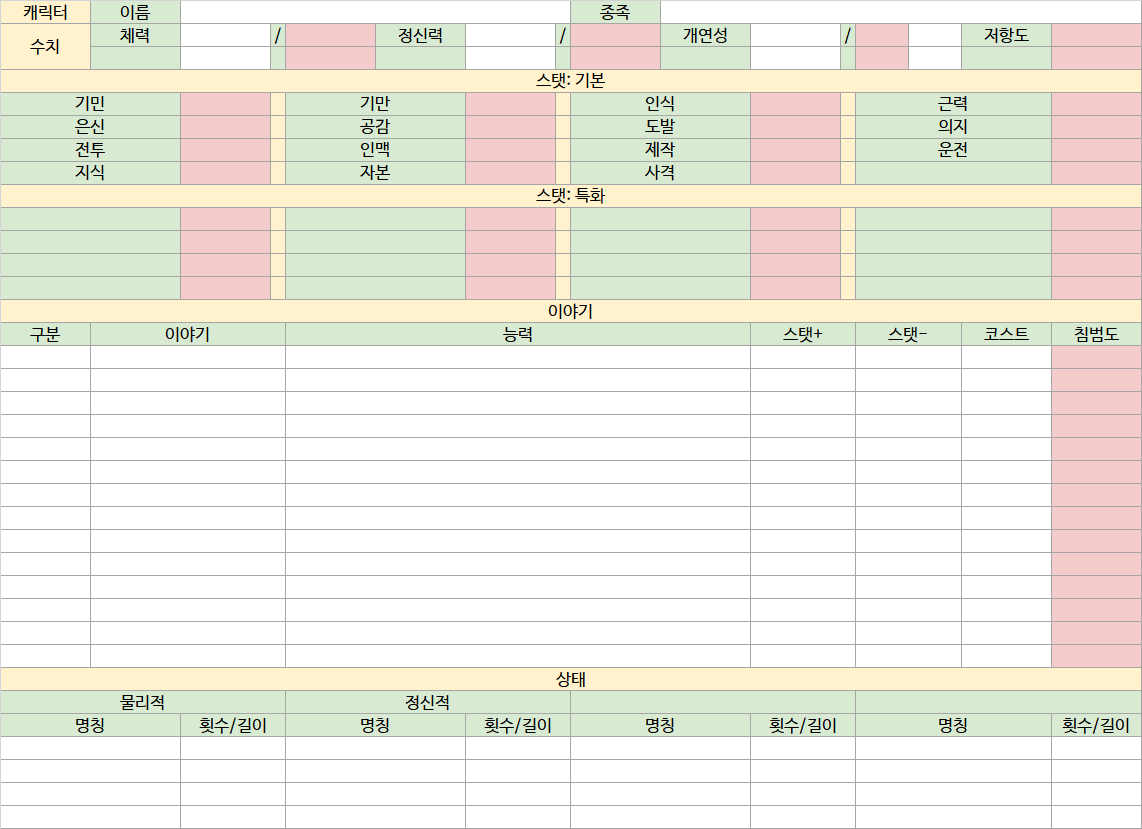
\includegraphics[width=\textwidth]{./Chapters/WoS/sheets/base.png}
	
	\section*{카토(Kato)}
		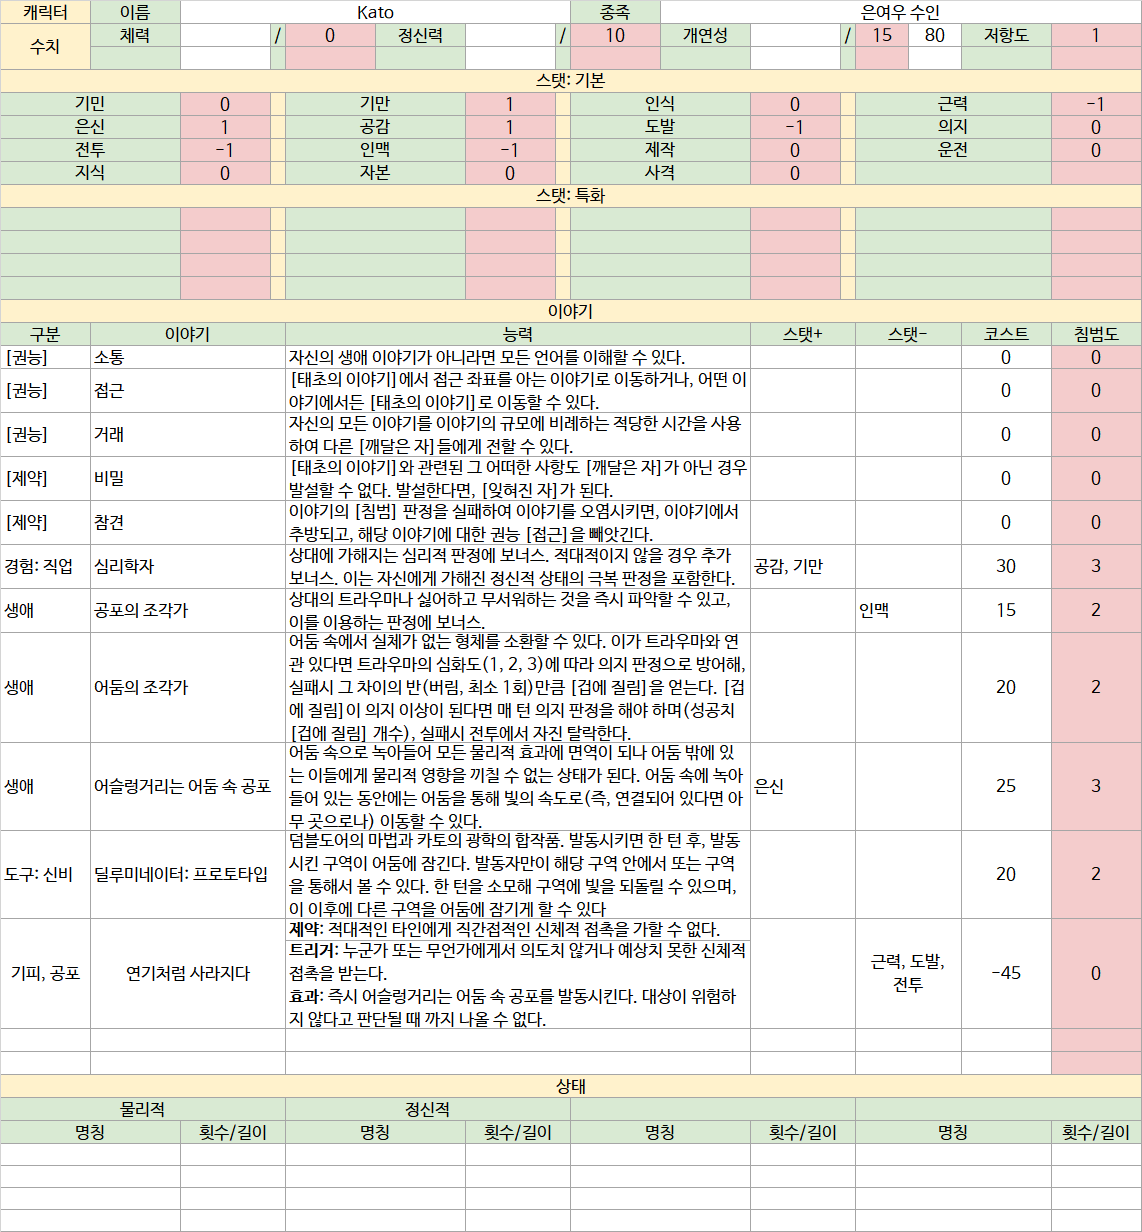
\includegraphics[width=\textwidth]{./Chapters/WoS/sheets/kato.png}
	
	\section*{네모(Nemo)}
		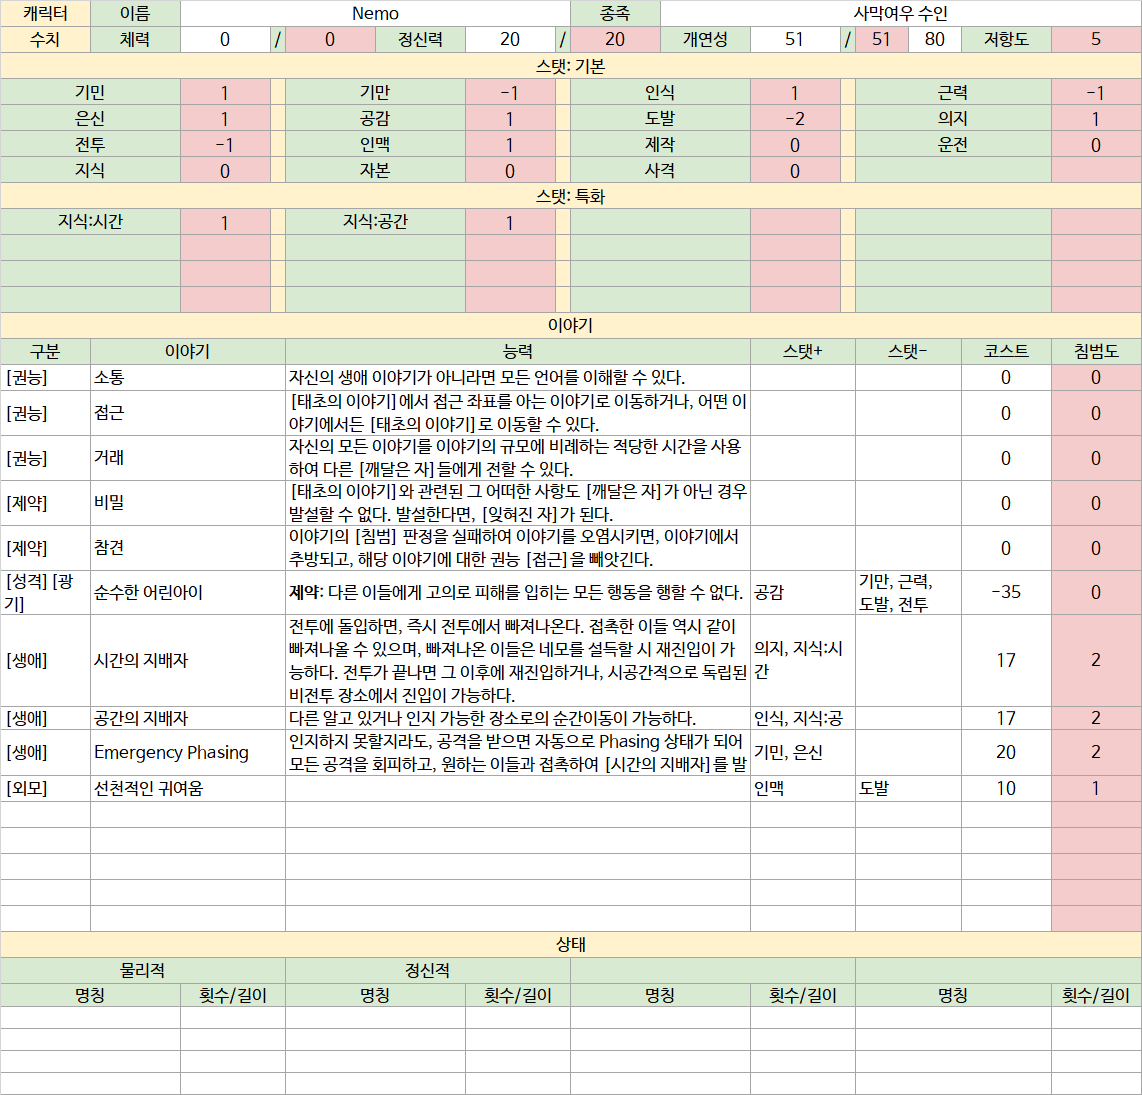
\includegraphics[width=\textwidth]{./Chapters/WoS/sheets/nemo.png}
	
	\section*{퓨어(Pure)}
		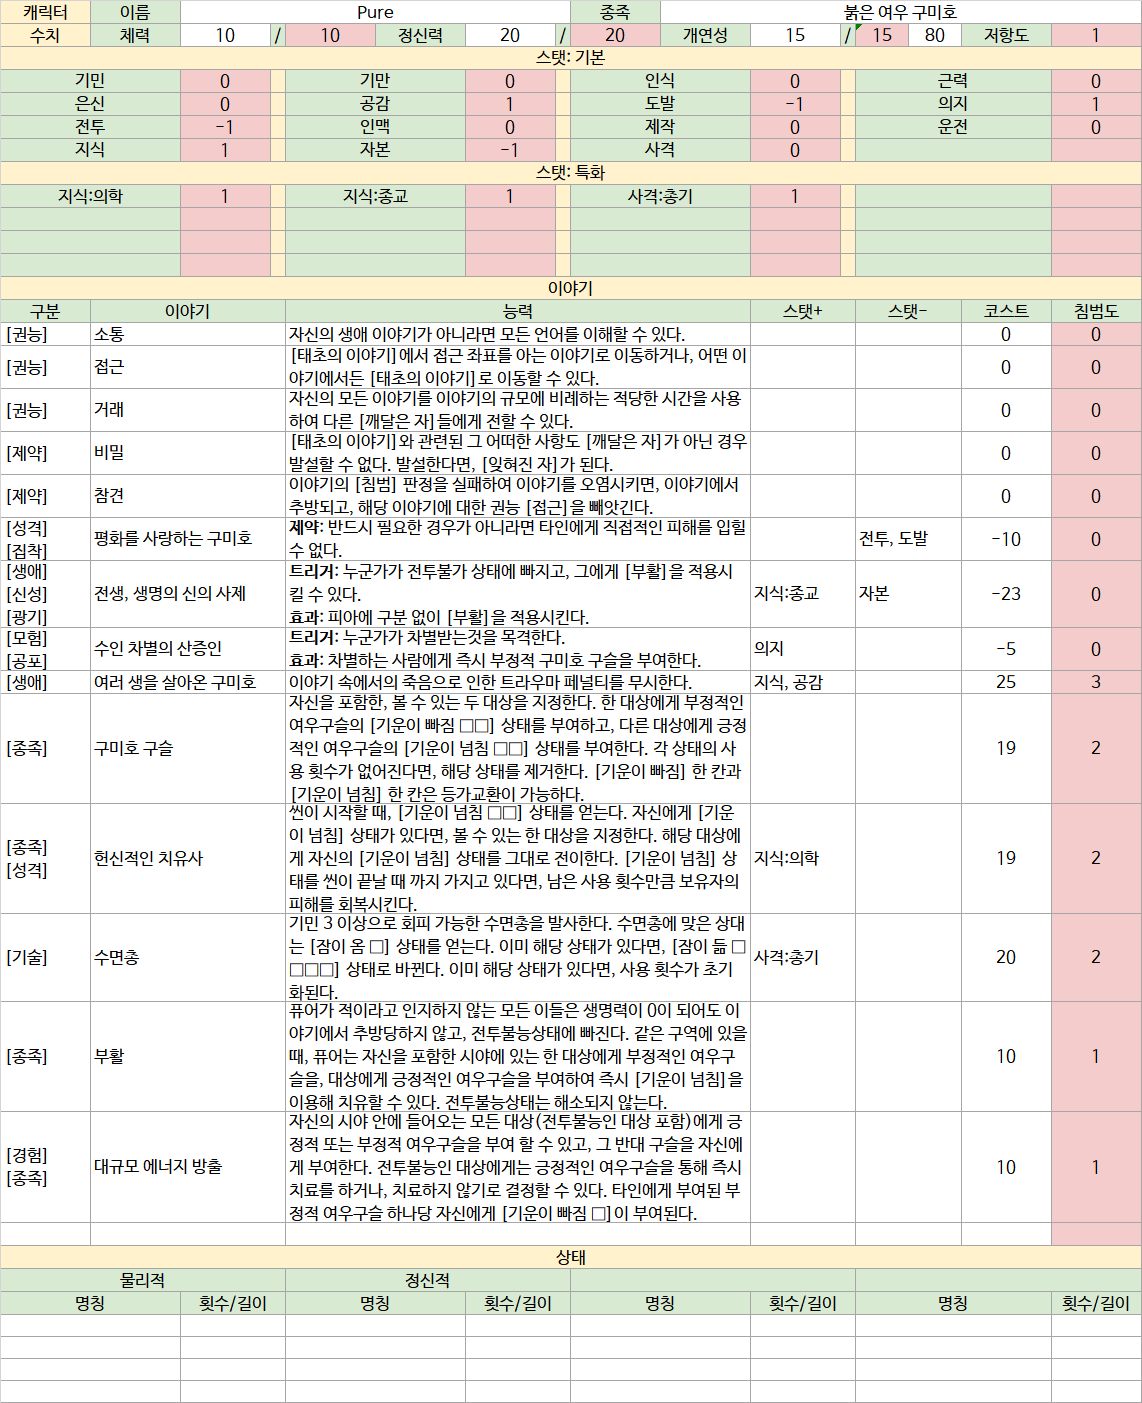
\includegraphics[width=\textwidth]{./Chapters/WoS/sheets/pure.png}
	
\end{document}
	
	\chapter{서사 속에서의 역할과 이야기}
		\documentclass{report}

\begin{document}
		\world{서사 속에 들어가면 여러분은 여러가지 역할과 이야기를 받게 됩니다. 어떤 경우에는 서사 속에 들어갔을 때 받게 될 이야기를 선택할 수 있는 경우도 있을 것이고, 어떤 경우에는 서사의 시공간적 배경으로 인해 강제로 이야기를 받게 되거나, 여러분이 가지고 있는 이야기가 변형될수도 있습니다.}
	
	서사 속에 들어간 이야기꾼들은 서사 속의 역할에 맞추어 추가적인 이야기를 받을 수 있습니다. 이 새로운 역할은 처음부터 주어지기도 하며, 나중에 필요에 의해 지급되거나 자신이 선택할 수도 있을 것입니다. 이 역할들은 간단하게 이야기만을 주기도 하지만, 새로운 능력이나 트라우마, 행동 제약 등을 제시할 수도 있습니다. 간단한 예시로, 사진 작가인 이야기꾼이 사진기가 발명된 직후의 이야기에 카메라를 들고 들어간다면 카메라가 커다란 구형 카메라로 변한다거나 하는 페널티가 생길 수 있을 것입니다.
	
	\bigskip
	
	보다 구체적인 예시로, 이야기꾼이 생명을 지켜야 하는 신성한 직업인 사제가 된 경우, 다음 이야기들을 부여할 수 있습니다:
	
	\begin{story}{깨어난 자}{[역할:사제][신성]}
		\entry{어떤 상황에서도 이성을 잃지 않는다.}
		
		\entry{모든 물리 공격에 [신성] 속성이 추가되어 타락한 자들에게 추가 정신력 또는 체력 피해를 준다.}
		
		\entry[\hline]{“비폭력"이 아닌 다른 트라우마의 트리거 조건을 만족했을 때 4df를 굴려 해당 트라우마의 트라우마 단계(기피 1, 공포 2, 광기 3) 이상의 수치가 나오면 효과를 무시한다.}
	\end{story}
	
	\begin{story}{비폭력}{[역할:사제][기피][공포]}
		\triggertrauma{기피}{생명체에게 피해를 입힌다.}{이번 씬 동안, 추방된다. “사제” 역할을 잃는다.}
		
		\triggertrauma[\hline]{공포}{생명체를 사망에 이르게 한다.}{이 서사에서 영구히 추방된다. “사제” 역할을 잃는다.}
	\end{story}
	
	역할이 이야기를 부여하는 것 외에도, 서사 속에 들어가면 그 서사에 맞는 이야기들이 강제로 적용될 수 있습니다. 예를 들어, 불안정한 공간에서 벌어지는 서사라면 다음 이야기가 부여될 수 있을 것입니다:
	\begin{story}{비정형의 공간}{[공간]}
		\entry[\hline]{우주 상에 떠다니는 불규칙한 공간이기 때문에 명중 또는 회피 판정을 할 때에는 별도의 해당 페널티를 상쇄할 만한 이야기가 없다면 명중/회피 페널티로서 4df를 굴려 해당 수치를 판정치에 반드시 더해야 한다.}
	\end{story}
	
	다른 많은 규칙에 존재하는 클래스 규칙을 사용하고 싶다면, 사용할 수 있습니다. 물론 이 이야기는 하나의 예시일 뿐이라는 것을 기억하세요:
	\begin{story}{클래스}{[세계]}
		\entry[\hline]{각 이야기꾼은 이 서사에 돌입하면 클래스 [물리] [마법] [신성] 중 한가지와 해당 클래스의 서브클래스 셋 중 하나를 선택하고, 해당 서브클래스 이야기의 능력과 제약을 받는다.
		
		\begin{tabularx}{0.97\textwidth}{X!{\color{black}\vrule}X!{\color{black}\vrule}X}
			\multicolumn{1}{c!{\color{black}\vrule}}{\textbf{[물리]}} & \multicolumn{1}{c!{\color{black}\vrule}}{\textbf{[마법]}} & \multicolumn{1}{c}{\textbf{[신성]}} \\ \hline
			\textbf{[Rogue] 도둑의 미덕} & \textbf{[Conjurer] 힘이 흘러넘쳐} & \textbf{[Cleric] 의심스러운 믿음} \\
			{자신을 인지하지 못한 이에 대한 판정 +2, 자신을 인지한 이에 대한 피해량 1 감소(최소 1)} & {원소마법 계열의 능력의 위력 증가(피해 1 증가, 치유 1 증가, 유틸기 포함), 쿨다운 1턴 증가.} & {모든 능력의 치유량 50\% 증가, 최대 체력 20\% 감소.} \\\hline
			\textbf{[Barbarian] 나 아프다!} & \textbf{[Arcana] 미래를 보는 눈} & \textbf{[Paladin] 올곧은 의심} \\ 
			{생명력이 최대 생명력의 50\% 미만일 때 가하는 근접 공격 피해 50\% 증가, 지능 관련 판정 -1} & {조준 또는 회피를 할 때 행운 사용시 두 번 굴려 그 중 원하는 수치로 판정, 회피 실패시 받는 피해량 50\% 증가.} & {집중해야 하는 기술에 관련된 판정에서 위력 50\% 증가, 집중력 판정에 -1} \\ \hline
			\textbf{[Ranger] 흔들림 없는 손} & \textbf{[Diablerie] 계약의 흔들림} & \textbf{[Druid] 어색한 대자연} \\ 
			{명중 판정에 행운 사용시 +1} & {모든 능력의 체력 소모량 50\% 감소(최소 1), 위력 감소(피해 1 감소, 치유 1 감소, 유틸기 포함)} & {자연과 소통을 통해 사용하는 능력들이 발동하는데에 1턴 추가로 걸림, 위력 50\% 증가.}
		\end{tabularx}
		}
	\end{story}
	
	이처럼 서사 속에서 역할을 부여받으면 그 역할에 맞는 이야기와 능력을 얻음으로서 해당 이야기의 세계를 보다 생생하게 체험하게 해 줄 수 있습니다.
	

\end{document}
	
	\chapter{판정과 이야기}
		\documentclass{report}

\begin{document}
	\world{여러분이 서사 속으로 들어가면 대부분은 개연성에 의해 서사 속의 등장인물로서 편입이 되게 됩니다. 이런 서사 속에서는, 여러분이 가지고 있는 이야기들의 도움을 받아야만 합니다. 여러분의 이야기는 여러분이 어떤 것을 잘 할 수 있고 어떤 것을 잘 하지 못하는지를 대변해줄 수 있을 뿐 아니라, 여러분이 어려운 상황에 처했을 때 직접적으로 도움을 줄 수도 있을 것입니다.}
	
	서사 속에서 이야기꾼들이 행동을 할 때, 자신이 가진 스탯과 이야기의 도움을 받을 수 있습니다. 임무의 성공 여부는 보통 스탯의 수치로 결정되지만, 이야기의 도움을 받을 수도 있고, 특정 이야기가 해당 상황을 [재현] 할 수 있다면, 자동으로 성공하거나 큰 도움을 받을수도 있습니다.
	
	\bigskip
	
	이야기꾼의 세계에서는 이야기별로 다른 판정 방법을 사용할 수는 있겠지만, 스탯을 사용하고 이야기의 도움을 받는 등의 기본적인 판정을 할 때에는 기본적으로 주사위를 사용하지 않습니다. 하지만 아래의 선택 규칙인 [행운] 규칙을 사용할 때에는 "퍼지 다이스(fudge dice)"라고 불리는 주사위를 사용합니다. 퍼지 다이스는 +, 0, -의 세 가지 종류의 면이 같은 수로 존재하는 주사위입니다. 주사위를 새로 구매할 수도 있지만, 보통 많이 소지하고 있을 d6을 사용하여 1\textasciitilde2는 -, 3\textasciitilde4는 0, 5\textasciitilde6은 +로 취급하는 방법이 있습니다. 이 주사위를 사용하기로 선택한 이유는 평균이 0이고 분산이 작기 때문에 주사위 굴림의 운보다는 스탯 수치가 더 큰 영향을 주기 때문입니다. 반면, 능력의 경우에는 시스템이 허용하는 그 어떤 판정 방법을 사용해도 무방합니다. 예를 들어 d4, d6, d8, d10, d12, d20, d\%\footnote{d100으로도 알려져 있다.} 등의 다른 주사위들이나 플레잉카드, 타로카드 등의 카드들을 이용한 판정을 사용하는 능력을 만들었다면 시스템의 허가 하에 사용할 수 있을 것입니다.
	
	\bigskip
	
	이야기의 도움을 받을 때에는 이야기의 내용에 해당 상황에 도움이 되는 속성이 포함되어야 합니다. 예를 들어서, 무거운 돌을 옮겨야 한다면 “헤라클레스의 가호를 받은 자”라는 이야기는 도움을 줄 수 있지만, “여러 생을 살아온 구미호”라는 이야기는 도움을 줄 수 없을 것입니다.
	
	이야기의 도움을 통해 (해당 상황에 사용되는 스탯)+(도움을 준 이야기 수)가 성공치보다 얼마나 높거나 낮은지에 따라 다음이 일어납니다:
	\begin{itemize}
		\item \textbf{3 이상 작다}: 실패합니다. \emph{대실패}로 판정되어, 해당 상황에 대한 해소 전까지 지속되는 부정적 상태를 하나 받습니다.
		\item \textbf{1\textasciitilde2 작다}: \emph{실패}합니다. 단, 시스템이 지정해주는 페널티(대표적으로 1회 사용 후 소멸되는 부정적 상태)를 받는다면 성공할 수 있습니다.
		\item \textbf{같거나 1 크다}: \emph{통과}합니다. 원하는 바를 이룰 수 있으나, 그 이상도 이하도 일어나지 않습니다.
		\item \textbf{2\textasciitilde3 크다}: \emph{성공}합니다. 추가적으로, 1회 도움을 받은 후 소멸되는 긍정적 임시 상태를 받습니다.
		\item \textbf{4 이상 크다}: 성공합니다. \emph{대성공}으로 판정되어, 상태가 해소되기 전까지 계속해서 도움을 받을 수 있는 긍정적 상태를 받습니다.
	\end{itemize}
	상태를 받을 때에는 어떤 상태인지 시스템과 플레이어 양쪽이 모두 제안할 수 있습니다. 만약 부정적이든 긍정적이든 상관 없이 상태를 받을 수 있는 판정에도 불구하고 누구도 받을만한 상태를 생각할 수 없는 경우, 상태를 받을 수 없습니다.
	
	\section*{임시 상태}
	임시 상태란 길게는 해당 세션동안, 짧게는 한두번정도의 도움을 받을 수 있는 잠시동안 지속되는 상태입니다. 이는 여러가지 방법으로 받을 수 있으며, 특정 임시 상태를 부여하는 능력이 존재할 수 있습니다. 임시 상태는 그 효과에 따라 긍정적, 부정적, 중립적의 세 가지로, 그 종류에 따라 물리적, 정신적 등으로 구분됩니다. 종류에 따른 구분 방식은 이 외에도 여러가지가 있을 수 있으며, 한 이야기의 분류는 절대적이지 않을 수 있습니다. 예를 들어 [잠이 옴]이라는 상태는 일반적인 상황에서라면 부정적인 상태일지라도, 며칠간 잠을 자지 못한 불면증 환자에게는 축복과도 같은 긍정적인 상태로 다가올 수 있습니다.
	
	상태들은 효과나 종류에 상관없이 존재하는 동안은 이야기처럼 활용되어 판정에 도움을 줄 수 있습니다. 각 상태는 해소되기 전까지는 계속하여 유지되는데, 이를 해소하는 방법은 다음과 같습니다:
	\begin{itemize}
		\item 횟수가 제한된 상태의 경우, 횟수의 소모
		\item 시간이 제한된 상태의 경우, 시간의 흐름
		\item 치료, 상담 등으로 인한 상태의 직접적 해소
		\item 환경으로 인해 일어난 상태의 경우, 해당 환경에서 벗어나거나 환경의 해소
	\end{itemize}
	
	\hypertarget{emersion}{}
	\section*{이야기의 [재현]}
	[재현]이란, 이야기 속의 상황과 현재 상황이 매우 유사한 경우 발생하는 예외사항입니다. 상황의 유사성에 따라 다음 중 하나가 선택적으로 적용됩니다:
	\begin{itemize}
		\item 어떤 상황을 극복해야 하는 경우:
		
		\begin{itemize}
			\item 상황이 세부 사항을 제외하고 거의 같은 경우, 자동으로 성공합니다.
			\item 상황에 유사성에 따라, 이야기의 도움을 크게 받아 한 번 이상의 도움을 받은 것으로 취급할 수 있습니다. 이 수치는 상황의 유사도에 따라서 시스템이 결정합니다.
		\end{itemize}
		
		\item 다른 이야기꾼와 대결하는 경우:
		
		\begin{itemize}
			\item 상황이 세부 사항을 제외하고 거의 같으며, 그 이야기에서도 해당 이야기꾼과 대결했었던 경우, 상대가 이와 동급의 이야기로 대항하지 않는다면 자동으로 성공합니다.
			\item 상황에 유사성에 따라, 이야기의 도움을 크게 받아 한 번 이상의 도움을 받은 것으로 취급할 수 있습니다. 이 수치는 상황의 유사도에 따라서 시스템이 결정합니다.
		\end{itemize}
	\end{itemize}
	예를 들어, 12과업을 행한 헤라클레스의 경우 \textbf{[네메아의 사자를 죽인 자]}라는 이야기를 가지고 있다면 다른 사자에 대한 대항 판정에 있어 자동으로 성공할 수 있고, 다른 맹수에 대한 대항 판정에 있어 자동으로 성공하지는 않겠지만 큰 보너스를 받게 될 수 있습니다. 만약 호랑이와 같이 사자와 유사한 맹수라면 +4 등 큰 보너스를, 악어와 같이 조금 거리가 있는 맹수라면 +2 등 작은 보너스를 받게 될 것입니다.
	
	\section*{이야기 효과의 우선순위}
	이따끔씩 여러 이야기가 한번에 적용되어야 할 때가 있을 수 있습니다. 예를 들어, 어떤 사건으로 인해 한 공포증의 트리거가 발동됨과 동시에 다른 패시브 능력의 조건이 충족된다거나 하는 식으로 말이죠. 이 경우에는, 다음과 같은 순서로 이야기의 우선순위가 정해집니다:
	\begin{enumerate}
		\item 이야기꾼이 들어가있는 세계 출신의 이야기
		\item 개연성 비용의 절대값이 높은 이야기
		\begin{itemize}
			\item 단 양수인 이야기와 음수인 이야기가 있다면, 양수인 이야기가 우선됨
		\end{itemize}
		\item 해당 이야기와 가장 관련 있는 이야기꾼의 스탯이 높은 이야기
		\begin{itemize}
			\item 기본적으로 스탯을 올려주는 이야기의 경우 해당 스탯, 또는 그 중 가장 높은 스탯
			\item 아닌 경우라 할지라도 이야기와 관련있는 스탯이 있다면 해당 스탯
			\item 전혀 없다고 생각된다면 이야기꾼의 의지 스탯을 이용함.
		\end{itemize}
		\item 위 모두가 동률이라면:
		\begin{itemize}
			\item 전투 상황이 아닐때, 
			\begin{itemize}
				\item 서로 다른 두 이야기꾼의 이야기라면 주사위를 굴려 결정.
				\item 한 이야기꾼의 이야기라면 이야기꾼의 마음대로 결정.
			\end{itemize}
			\item 전투 상황이라면 더 빠르게 자신의 턴이 돌아오는 이야기꾼의 이야기부터.
			\subitem 현재 턴인 이야기꾼 $\rightarrow$ 다음 턴인 이야기꾼 $\rightarrow$ ...
		\end{itemize}
	\end{enumerate}
	
	
	\section*{\hypertarget{pow-of-luck-unluck}{(선택 규칙)``행운"의 힘과 ``불운"의 힘}}
	다음 중 전부 또는 일부를 선택하여 적용시킬 수 있습니다:
	\begin{itemize}
		\item 모든 행동을 할 때, ``행운"의 힘을 빌리기로 결정할 수 있습니다. ``행운"의 힘을 사용하고자 한다면, 이야기의 도움을 받은 횟수에 퍼지 주사위 네 개를 굴려 나온 값을 더해 판정합니다.
		
		\begin{itemize}
			\item ``행운"을 사용한다면, 반드시 모든 판정에 ``행운"을 적용시키기로 결정할 수 있습니다.\footnote{사실 이렇게 하는 것이 조금 더 긴장감을 유발할 수 있기도 합니다.}
			
			\item ++++은 대성공, -{}-{}-{}-는 대실패로 판정을 지정할 수도 있습니다. 이 경우, 판정의 결과 수치에 상관없이 ++++ 또는 -{}-{}-{}-가 나오는 경우 대성공 또는 대실패합니다.
		\end{itemize}
		
		\item 세계 간의 괴리감과 함께 ``불운의 힘"이 깃들어 ``재현"이 실패할 확률이 존재할 수 있습니다. 이 경우, 퍼지 주사위 네 개를 굴립니다. 만약 -{}-{}-{}-가 나온다면, 이 이야기를 일반적인 이야기의 도움으로 취급합니다. -{}-{}-{}-가 나오지 않는다면, ``재현"이 정상적으로 수행됩니다.
	\end{itemize}

	\ifprintout\else
	서플리먼트의 \hyperlink{story:luck-unluck}{행운과 불운} 챕터의 이야기들과 같은 이야기로 구현할 수 있습니다.
	\fi
	
	\section*{판정의 예시\footnote{애스크를 통해 질문 주신 익명의 질문자분께 감사드립니다.}}
	
	예를 들기 위해 인식이 1인 이야기꾼이 있고, 어두운 통로에서 무언가 빠르게 휙 지나가는 것을 보기 위해 성공치가 4인 인식 판정을 해야 한다고 가정하겠습니다.
	
	이 이야기꾼에게 만약 [야간시]와 같은 어두운 곳에서 보는데에 도움을 주는 이야기나, [야구선수]와 같이 빠른 속도로 지나가는 물체를 보는데에 도움을 주는 이야기가 있다면, 이들로 인해 판정치에 각각 +1을 받을 수 있습니다. 이 경우 판정치, 즉 [(스탯)+(이야기)]는 3이 됩니다. 보통의 경우라면 성공치가 4이므로 1 차이로 이야기꾼은 인식 판정에 실패하거나, [눈이 아픔]과 같은 짧게 유지되는 임시 상태를 받음으로서 판정에 성공하게 될 수 있습니다. 즉, 기본적으로 판정을 할 때에는 다이스를 사용하지 않습니다. 오로지 이야기꾼의 스탯과 이야기, 즉 그들의 실력으로 판정이 결정되는 것이죠.
	
	하지만 [행운] 규칙을 사용하는 경우 퍼지 다이스 4개를 굴려 ``행운"의 힘이 이야기꾼의 판정에 개입하도록 할 수 있습니다. 이 경우 판정치에 퍼지 다이스 네 개를 굴린 결과를 더한 것이 판정치가 됩니다. 예를 들어 위의 상황에서 [행운]의 힘을 빌렸을 때, 퍼지 다이스의 결과가 -{}-0+(-1)이라면 판정치는 2가 되어 실패하게 되나, 0++0(+2)라면 판정치는 5가 되어 ``운이 좋게도" 열쇠를 물고 있는 쥐 한마리가 빠르게 지나갔다는 것을 보게 될수도 있게 되는 것이죠.
	
	만약 이 경우에 적용 가능한 능력이 존재한다면 상황은 역시 달라질 수 있습니다. 만약 위의 이야기 중 [야간시]가 다음과 같은 능력을 가지고 있다고 가정해봅시다:
	\begin{story}{야간시}{[종족]}
		\entry{어두운 곳에서 모든 판정을 할 때에 +1을 받는다. 특히, 시각에 의존한 판정을 할 때에 추가로 +1을 받는다.}
	\end{story}
	이 경우, 판정치는 3에 [야간시]의 능력에 의한 +2가 추가되어 ``행운"의 힘 없이도 5의 판정치로 판정에 성공하게 됩니다.
	

\end{document}
	
	\chapter{전투}
		\documentclass{report}

\begin{document}
	전투 상황에서는, 기민 스탯이 더 높은 이야기꾼이 먼저 턴을 가집니다. 한 턴은 5초로 계산하므로, 간단한 행동 한가지 정도만을 할 수 있습니다. 각 턴은 다음과 같이 진행됩니다:
	\begin{itemize}
		\item \textbf{결정}: 행할 행동을 결정합니다. 해당 행동에 가지고 있는 이야기 중 도움이 되는 이야기들과 능력의 도움을 받을 수 있습니다.
		\item \textbf{반응}: 주변의 이야기꾼들이 이 행동을 돕거나 방해할 수 있습니다.
		\begin{itemize}
			\item \textbf{행동의 대상}: 행동의 대상은 자신의 모든 이야기와 능력을 활용하여 해당 행동을 돕거나 방해할 수 있습니다.
			\item \textbf{나머지 이야기꾼}: 행동의 대상이 아닌 이야기꾼은 자신의 능력들은 모두 활용할 수 있으나, 자신의 이야기를 최대 한개까지만 활용하여 해당 행동을 돕거나 방해할 수 있습니다. 단, 이 이야기로 인하여 자동 성공을 결과로 가지게 할 수 없으며, 다음 자신의 턴의 행동이 완료되기 전까지는 돕는데 사용한 이야기의 도움은 받지 못합니다.
		\end{itemize}
		\item \textbf{결과}: 해당 행동의 결과를 판정합니다.
	\end{itemize}
	기본적으로는 도와준 이야기의 규모에서 방해한 이야기의 규모를 뺀 값의 피해만큼을 행동의 대상에게 줍니다.
	
	가하는 피해가 2 이상일때에는 가하는 피해를 2 줄이고, 다음과 같은 일을 할 수 있습니다:
	\begin{itemize}
		\item 무기를 떨어뜨리도록 만들거나, 넘어뜨리거나 하는 등 상대에게 부정적인 상황 하나를 만들기로 결정하거나
		\item 1회 사용 가능한 부정적인 상태를 주도록 선택할 수 있습니다.
	\end{itemize}
	이 상황과 상태는 공격자가 결정하며, 한 공격에 피해량이 충분하다면 여러번 사용할 수 있습니다.
	
	피해를 받을 때에는 먼저 물리 피해의 경우 체력, 정신 피해의 경우에는 정신력에 피해를 받습니다. 만약 체력 또는 정신력이 0인 경우, 해당 수치만큼이 개연성에서 감해집니다.
	체력과 정신력은 씬이 종료될 때 마다 회복됩니다. 하지만 개연성은 회복되지 않습니다. 다만, 체력 또는 정신력을 회복시키는 능력에 의해서는 각각 해당 수치가 최대치인 경우 개연성이 회복될 수 있습니다. 이 이외의 방법으로 개연성을 회복시킬 수 있는 방법은 서사에서 추방되었다가 다시 진입하여 개연성을 초기화하는 방법뿐입니다.
	개연성이 0이 되면, 서사에서 추방됩니다. 자세한 내용은 \hyperlink{intrusion}{이야기의 [침범] 판정}을 확인하세요.
	
	\section*{지형}
	지형은 “구역”으로 구분되어 있습니다. 전투 상황에서 이동을 할 때에는 한 턴에 한 구역까지 이동할 수 있으며, 기본적으로 같은 구역 내에 있는 캐릭터 끼리는 서로 주먹, 칼 등의 근접 무기로 공격을 할 수 있습니다. 구역별로 특이사항이나 상태, 이야기를 가지고 있을 수 있습니다.
	

\end{document}
	
	\hypertarget{trauma}{}
	\chapter{트라우마}
		\documentclass{report}

\begin{document}
	이야기꾼들은 여러가지 정신적인 후유증을 가지고 살아갑니다. [기피], [공포], [집착], [중독], [광기]가 바로 그것입니다. [기피]가 심화되면 [공포]가, [공포]가 심화되면 [광기]가 됩니다. 중독증이나 집착증 등은 트라우마로 보기 어려우나, 트라우마와 동일하게 취급됩니다. 이 경우 [기피], [공포] 단계 대신 [집착], [중독] 단계를 사용합니다. [광기] 단계는 유지됩니다. 어떤 후유증은 일시적일수도 있고, 직접 해소될 방법이 있을 수도 있습니다.
	
	이들은 기본적으로 다음과 같은 형식으로 이루어집니다:
	
	\begin{itemize}
		\item \textbf{트리거}
		\subitem 트라우마를 발동시킬 조건입니다. 이 조건을 충족시키면, 효과가 발동됩니다.
		
		\item \textbf{효과}
		\subitem 트라우마로 인해 발동되는 효과입니다. 이 효과에 대한 예시로는 다음이 있습니다:
		\begin{itemize}
			\item 일정 시간동안 특정 부정적인 상태를 얻습니다.
			\item (피아 구분 없이) 무작위 대상을 공격합니다.
			\item 아군을 공격합니다.
			\item 피아의 구분을 할 수 없게 됩니다.
			\item 주변 상황이 어떻든 상관없이 트리거를 없애고자 합니다.
			\item 일정 시간동안 공격을 방어하지 못합니다.
			\item 그 상황에서 어떻게든 빠져나가려고 합니다.
		\end{itemize}
	\end{itemize}
	
	캐릭터의 행동을 제약시키는 조건만 존재하는 트라우마 역시 가능하며, 트리거/효과와 함께 제약이 같이 존재할 수 있습니다. 제약만 있는 트라우마의 경우, 제약 자체가 트리거와 효과의 역할을 함께 해야 한다는 점을 고려해 제약을 정하시면 됩니다.
	
	\section*{트라우마의 심각도}
	
	트라우마의 심각도는 그 효과에 따라 다음과 같이 결정하면 됩니다:
	
	\smallskip
	
	\begin{tabularx}{\textwidth}{c!{\color{black}\vrule}X}
		\hline
		\textbf{심각도} &
			\textbf{기준}\\ \hline \hline
		
		[기피], [집착]  &
		\makecell[l]{
			\begin{tabularx}{\linewidth}{X}
				제약사항은 없으나 이야기꾼의 서사를 풍부하게 하기 위한 장치\footnote{단, 이를 너무 남발할 경우 개연성이 과도하게 흘러넘칠 수 있으므로 한 이야기꾼당 한개 정도로 제한하는 것을 추천합니다.}\\\hline
				비전투시의 행동 제약이며, 주의를 조금만 기울여도 발동되지 않을 수 있는 효과이거나, 발동되더라도 큰 제약이 되지 않는 효과
			\end{tabularx}
		}\\\hline
		
		[공포], [중독]  &
		\makecell[l]{
			\begin{tabularx}{\linewidth}{X}
				비전투시의 행동 제약이며, 주의 여부에 상관없이 발동될 수 있는 효과이며, 발동되었을 때 이야기꾼의 사고나 행동을 뒤바꿀 수 있는 효과\\\hline
				전투시의 행동 제약이며, 주의를 조금만 기울여도 발동되지 않을 수 있는 효과이거나, 발동되더라도 큰 제약이 되지 않는 효과
			\end{tabularx}
		}\\\hline
		
		[광기]          &
		\makecell[l]{
			\begin{tabularx}{\linewidth}{X}
				비전투시의 행동 제약이며, 주의 여부에 상관없이 발동될 수 있는 효과이며, 발동되었을 때 이야기꾼 본인 뿐 아니라 주변인의 사고와 행동 등에도 영향을 끼치는 효과\\\hline
				전투시의 행동 제약이며, 주의 여부에 상관없이 발동될 수 있는 효과이며, 발동되었을 때 이야기꾼의 사고나 행동을 뒤바꿀 수 있는 효과
			\end{tabularx}
		}\\\hline
	\end{tabularx}
	
	\smallskip
	
	두 가지 이상에 해당한다면 더 낮은 쪽의 심각도를 따릅니다. 가령, 전투, 비전투를 가리지 않고 주의를 기울인다면 발동되지 않을 수 있는 트라우마의 경우 [기피] 또는 [집착] 단계의 심화도를 가진 트라우마가 됩니다.
	
\end{document}
	
	\hypertarget{intrusion}{}
	\chapter{이야기의 [침범] 판정}
		\documentclass{report}

\begin{document}
	\world{이야기꾼이 자신의 출신 서사가 아닌 서사에 들어갔을 때, 여러분은 서사의 외부자로서 서사의 흐름을 방해하거나 오염시켜서는 안됩니다. 서사가 오염되었다는 것은 서사 자체가 사라졌다는 것이 아니라, 그 서사의 간섭받지 않은 결말, 즉 [종장]이 희석되어 알아보기 힘들게 되었다는 것을 의미합니다. 이렇게 되면 그 서사의 본질이 바뀌게 되는 것이죠. 이를 막기 위해 [참견]의 제약으로, 너무 서사에 큰 손상이 우려될 때에는 이야기꾼을 서사에서 추방하게 됩니다.}
	\world{여러분은 서사 속에서 저를 도와 서사의 흐름을 되돌리는 과정에서 그 서사 속에서의 죽음을 맞이하게 될 수도 있습니다. 하지만, 이는 그 서사 속에서 그 역할으로서의 당신이 죽었을 뿐이라는 것을 명심하세요. 새로운 역할을 부여받아 다시 서사 속으로 들어가는것은 당연히 가능합니다.}
	
	서사를 오염시키는 행동인지를 판단하기 위하여, 시스템은 행동에 따라 [침범] 판정을 하도록 강요합니다. 서사의 [운명]이나 지식을 거스르는 행동, 부여받은 이야기의 역할에 맞지 않는 행동, 서사에 어울리지 않는 능력을 사용하는 행동 등이 이에 포함됩니다.
	
	이야기꾼들이 가지고 있는 이야기들은 각각 개연성 코스트가 있습니다. 해당 이야기의 [침범도]는 개연성 코스트의 1/10(올림)으로 정의합니다.
	
	이야기꾼들에게는 각각 최대 개연성이 있습니다. 이야기꾼의 [저항도]는 최대 개연성의 1/10(버림)으로 정의합니다.
	
	\bigskip
	
	[침범] 판정은 판정을 할 때 마다 기본 난이도가 점점 증가합니다. [침범] 판정의 기본 난이도는 보통 최초에 -1으로 시작하여, 이야기꾼의 수만큼 판정을 할 때 마다 1씩 증가합니다. 다르게 생각하려면, 한 번 판정시마다 (1/이야기꾼)만큼 난이도가 상승한다고 생각해도 됩니다. 만약 누군가가 이야기를 이미 [침범]한 상태였다면, 시작할 때의 침범 판정의 난이도는 0보다 높을 수 있습니다. 이 기본 난이도에 침범 판정을 일으킨 이야기의 침범도를 더한 것이 난이도가 됩니다.
	
	[침범] 판정을 할 때에는 4df를 굴려 자신의 저항도를 더합니다. 이 값이 난이도보다 높으면 성공하고, 같거나 낮으면 실패합니다.
	
	[침범] 판정의 결과와는 상관 없이, 행동은 완료할 수 있습니다.
	
	[침범] 판정이 성공한다면 행동이 정상적으로 행해집니다.
	
	[침범] 판정이 실패한다면, 자신의 개연성을 해당 이야기의 개연성 코스트만큼 감합니다. 또는, 서사에 따라 독립적인 실패의 대가가 따를 수 있습니다. 가령 이야기의 끝에 다다르고 있는 서사는 오염될 가능성이 적기에, 다음 이야기의 내용으로 페널티가 대체될 수 있습니다:
	
	\begin{story}{시간의 끝}{[시간]}
		\entry{이 서사는 이미 시간의 끝을 향해 달려가고 있기 때문에 서사의 개연성을 해칠 염려가 매우 적다. 따라서, [침범] 판정에 실패할 때, 다음 씬(비전투) 또는 두 턴 후(전투)까지 해당 판정에 실패한 이야기가 전면 봉쇄되어, 기술 뿐 아니라 해당 이야기로부터의 도움도 받을 수 없다(단, 스탯은 유지된다). 개연성 판정 난이도의 초기화는 이야기의 봉쇄가 일어나면 즉시 일어나나, 이야기가 불안정해짐에 따라 판정이 일어날 때 마다 난이도가 1 상승한다.}
	\end{story}
	
	어떠한 방법으로든 개연성이 0이 된다면 서사에서 추방됩니다. 다음이 순서대로 진행됩니다:
	\begin{itemize}
		\item 개연성이 0이 된 이야기꾼이 서사에서 추방됩니다. 해당 씬은 그대로 진행됩니다.
		\item 앞으로 등장인물이 아닌 모든 이야기꾼은 모든 이야기를 사용하거다 도움을 받는데에 있어, 반드시 [침범] 판정을 해야 합니다.
		\item 해당 씬이 종료되면 자동으로 모든 이야기꾼이 서사에서 추방됩니다.
	\end{itemize}
	이야기꾼 vs 타락한 자의 경우, 시스템은 여러분이 돕고 있다는 사실을 알기에, 이 행위들을 적대 행위로서 간주하지는 않습니다. 시스템은 여러분의 권한을 다시 복구시켜 줄 것이며, 임무를 계속할 수 있습니다. 이로 인해 타락한 자가 추방되더라도 같이 추방되었기 때문에 일괄적으로 복구되어, 서사를 계속 어지럽히는데에 일조합니다.
	
	[침범] 판정의 난이도는 모든 이야기꾼이 추방된 이후 다시 초기화됩니다.
	
	\section*{세계관 출신 인물의 이야기에 의한 침범 판정}
	가끔 이야기의 [깨달은 자]가 아닌 등장인물 중에는 먼치킨스러운 능력을 보유하고 있는 경우가 있습니다. 또, 이야기꾼들은 자신의 출신 서사로 돌아가기도 하죠. 세계관과 연관 있는 이야기 또는 인물에 의한 [침범] 판정에 대한 세 가지 중요한 사실은 다음과 같습니다:
	\begin{enumerate}
		\item {}[깨달은 자]가 아닌 등장인물에 의해서는 [침범] 판정이 일어나지 않습니다.
		\item 그 세계 속에서 얻은 이야기 또는 능력에 의해서는 [침범] 판정이 일어나지 않습니다.
		\begin{itemize}
			\item 이는 누군가 개연성이 0이 되어 추방되었을 때의 강제 판정에도 포함됩니다.
		\end{itemize}
		\item 해당 세계관의 출신인 [깨달은 자]는 개연성이 0이 되어도 서사에서 추방되지 않습니다.
		\begin{itemize}
			\item 추방되는 대신, 제대로 된 치료를 받기 전까지 체력과 정신력이 회복되지 않고 행동불능 상태가 됩니다.
			\item 이로 인해 이야기꾼이 사망하는 경우도 생길 수 있습니다.
		\end{itemize}
	\end{enumerate}
	
	\section*{\hypertarget{the-story-continues}{(선택 규칙)계속되는 서사}}
	한 서사의 세계 속에서 여러 서사가 진행된다면, 서사가 끝난 이후에, [침범] 판정의 난이도를 확인하여 다음 서사에는 해당 난이도에서 [침범] 판정의 난이도가 시작하게 할 수 있습니다.
	
	서플리먼트의 \storyref{probability:the-story-continues}{계속되는 서사}와 같은 이야기로 구현할 수 있습니다.

\end{document}
	
	\hypertarget{growth}{}
	\chapter{이야기꾼의 성장과 죽음}
		\documentclass{report}

\begin{document}
	이야기꾼은 항상 변화하고, 성장합니다. 서사 속에서 죽음을 맞기도 하고, 서사 속에서 새로운 이야기를 얻으며 성장하기도 합니다.
	
	\section*{죽음}
	이야기꾼의 개연성이 0이 되면 해당 서사에서 죽음을 맞이하여, 추방됩니다. 해당 시점에서 다음이 모두 일어납니다:
	\begin{itemize}
		\item 죽은 원인 또는 상황에 대한 [기피]. 이미 유사한 [기피]나 [공포]가 있다면 해당 효과가 각각 [공포] 또는 [광기]로 심화됩니다. [광기]가 이미 있는 경우라 할지라도 관련 있는 새로운 트라우마를 얻거나 [광기]의 효과가 더 쉽게 트리거 되거나, 효과가 심화되는 등 페널티를 반드시 받습니다.
		\item 서사의 역할으로 인해 얻은 이야기를 모두 잃습니다.
		\item 받은 모든 임시 상태를 잃습니다.
		\item {}[태초의 이야기]에서 다시 나타납니다. 해당 씬이 끝난 뒤에, 재진입이 가능합니다.
	\end{itemize}
	
	\section*{미미한 성장}
	이야기꾼이 전투를 겪었거나, 이야기의 변화를 겪었다면 일어납니다. 시스템의 허가 하에 개연성을 소모하고 방금 있었던 전투나 변화에 어울리는 이야기 하나를 얻거나, 이미 존재하는 이야기 하나를 바꿀 수 있습니다. 미미한 성장으로 능력을 변화시키거나, 이야기를 잃을 수는 없습니다.
	
	\section*{작은 성장}
	서사 하나가 끝날 때 마다 이야기에서 얻는 보상과는 별개로 다음 중 하나를 할 수 있습니다:
	\begin{itemize}
		\item 개연성을 소모하고, 이야기를 하나 얻습니다.
		\item 개연성을 소모하고, 이미 있는 이야기에 대한 기술을 하나 얻습니다.
		\item 이야기 하나를 다른 이야기로 바꿉니다.
	\end{itemize}
	작은 성장과는 별개로, 서사에서 얻는 보상에 대한 가이드라인은 능력 가이드라인 챕터의 \hyperlink{reward}{서사의 보상} 부분을 참고하세요.
	
	\section*{중간 성장}
	시스템의 인정을 받는다면(보통 서사 두세개가 끝날때마다 한번) 다음을 모두 할 수 있습니다:
	\begin{itemize}
		\item 기본 최대 개연성 10을 얻습니다.
		\item 작은 성장을 합니다.\footnote{\label{medium-upgrade-small-upgrade}오타 아닙니다. 작은 성장의 선택지 중 한 가지를 선택해서 적용시키는 것을 두번 할 수 있습니다.}
		\item 작은 성장을 합니다.\footnoteref{medium-upgrade-small-upgrade}
	\end{itemize}
	
	\section*{큰 성장}
	시스템의 위기를 타파할 때 마다(보통 서사 대여섯개정도가 끝날때마다 한번) 다음을 모두 할 수 있습니다:
	\begin{itemize}
		\item 기본 최대 개연성 10을 얻습니다.\footnote{\label{big-upgrade-cost}즉, 기본 최대 개연성 20을 얻습니다.}
		\item 이야기와 그에 대한 기술을 하나 얻습니다.
		\item 중간 성장을 합니다.\footnoteref{big-upgrade-cost}
		\item 작은 성장을 합니다.
	\end{itemize}
	

\end{document}
	
	\hypertarget{ability-guidelines}{}
	\chapter{능력 가이드라인}
		\documentclass{report}

\begin{document}
	이야기에 따른 능력은 다양한 종류가 있을 수 있습니다.
	캐릭터의 서사에 따라서, 강력한 능력은 마나와 같은 자원을 소모할수도, 사용 대기 시간이 존재할수도, 시전 시간이 존재할수도, 사용 횟수 제한이 존재할수도, 까다로운 사용 조건이 존재할수도 있습니다. 하지만 모두 공통적으로, 다른 서사에 들어가면서 능력이 어느 정도 약화됩니다.
	이 장에서는 능력이 할 수 있는 일을 제시하고, 그 효과에 대한 범위에 대해 생각합니다.
	
	능력은 크게 [효과형], [활용형]으로 구분됩니다. 이 구분은 절대적이지 않습니다.
	
	[효과형] 능력은 아군 또는 적군에게 직접적으로 효과를 부여하는 등의 효과를 가진 능력입니다. 크게 [공격형]과 [지원형]으로 구분됩니다.
	[공격형] 능력은 상대에게 피해를 주거나, 기절 등 행동에 직접적인 제약을 주는 부정적인 상태를 주는 능력을 의미합니다.
	[지원형] 능력은 아군의 피해를 막거나 치유하고, 아군에게 도움이 되는 상태를, 적에게는 직접적인 제약이 되지는 않으나 능력 사용을 약화시키는 능력을 의미합니다.
	[효과형] 능력은 여러가지 속성을 가질 수 있습니다. 이 속성들은 능력의 성능과 개연성 비용에 직접적인 영향을 끼칩니다.
	
	아래의 수치는 성능에 따른 대략적인 개연성 비용입니다\ifprintout\footnote{3.0.0 버전의 최초 릴리스를 기준으로 적혀있습니다. 업데이트된 비용이나 이 이외의 비용이 필요하다면 \href{https://git.io/fjphB}{룰북}을 참고하시거나, 없다면 마음대로 판단하셔도 괜찮습니다. 정 모르시겠다면 제작자에게 문의해주셔도 괜찮습니다.}\fi:
	%개연성 비용	 밸런스 패치
	\begin{itemize}
		\item 피해
		\begin{itemize}
			\item \textbf{직접 피해(Direct Damage)}: 피해량 1이 증가할때마다 개연성 비용 3이 추가됩니다.
			\item \textbf{지속 피해(Damage over Time)}: 턴당 피해량이 1 증가할때마다 개연성 비용 2가 추가됩니다. 지속시간 1턴마다 개연성 비용 2가 추가됩니다. 단, 최대 줄 수 있는 총 피해량의 세 배보다 이 코스트가 적다면 최대로 줄 수 있는 총 피해량의 세 배의 코스트를 가집니다.
			\item \textbf{본인 피해(Self-inflicted Damage)}: 본인에게 가하는 피해량 1이 증가할때마다 개연성 비용 2가 감소합니다.
		\end{itemize}
		
		\item 회복/방지
		\begin{itemize}
			\item \textbf{피해의 방지(Prevention)}: 최대로 방지할 수 있는 피해량 1당 개연성 비용 2가 추가됩니다.
			\item \textbf{피해의 회복(Healing)}: 최대로 치유할 수 있는 피해량 1당 개연성 비용 4가 추가됩니다.
			\item \textbf{지속 회복(Healing over time)}: 턴당 회복량이 1 증가할때마다 개연성 비용 2가 추가됩니다. 지속시간 1턴마다 개연성 비용 2가 추가됩니다. 5턴 이상은 추가되지 않습니다.
		\end{itemize}
		
		\item 사거리
		\begin{itemize}
			\item 아래의 내용을 계산할 때, 구역의 배치를 한 변이 10m인 무한 격자형 구역으로 생각합니다.
			\item \textbf{사거리(Ranged)}: 최대 사거리까지 떨어진 구역 수당 개연성 비용 1이 증가합니다. 5 이상으로 증가하지 않습니다.
			\item \textbf{범위(Area of Effect)}: 범위에 포함되는 구역당 개연성 비용 2가 증가합니다. 단, 아군 피해(Friendly Fire) 혹은 적군 회복 등 의도치 않은 결과를 불러올 수 있는 능력은 이 효과를 받지 않습니다.
			\item \textbf{회피 가능성(Dodgeability)}
				\begin{itemize}
					\item \textbf{조준(Aim)}: 조준이 필요하다면 개연성 비용 4가 감소합니다.
					\item \textbf{경감 가능(Reducable)}: 피해의 경감이 가능하다면 개연성 비용 2가 감소합니다.
					\item \textbf{회피 가능(Dodgeable)}: 회피가 가능하다면 개연성 비용 4가 감소합니다.
					\item \textbf{대상 지정(Targeted)/회피 불가(Undodgeable)}: 조준이 불필요하며 회피가 불가능하다면 개연성 비용 3이 증가합니다.
				\end{itemize}
			\item \textbf{거리에 따른 피해량 감소(Damage Falloff)}: 한 구역당 감소되는 피해량이 1 증가할때마다 개연성 비용 1이 감소합니다.
		\end{itemize}
		
		\item 사용 빈도
		\begin{itemize}
			\item \textbf{자원(Resource)}: 자원을 사용하는 경우 개연성 비용 3이 감소합니다. 추가로, 자원이 자동으로 충전되지 않는 등 자원을 찾기 어렵다면 개연성 비용 2가 감소합니다.
			\item \textbf{횟수 제한(Limited Use)}: 개연성 비용 10이 감소합니다. 씬당 사용 가능 횟수 1회당 개연성 비용 1이 증가합니다. 씬당 10회 이상 사용할 수 있는 능력은 횟수제한이 없는 것으로 간주합니다.
			\item \textbf{조건(Condition)}: 조건의 달성 수준에 따라 개연성 비용 1\textasciitilde10이 감소합니다.
			\item \textbf{준비 시간(Cooldown)}: 기술의 준비 시간 1턴당 개연성 비용 1이 감소합니다.
			\item \textbf{충전(Charge time)}: 기술의 충전 시간 1턴당 개연성 비용 1이 감소합니다. 만약 충전 시간동안 다른 행동에 제약을 받는다면, 1씩이 추가로 감소합니다.
			\item \textbf{연속 사용(Consecutive Usage)}: 한 턴에 여러 번 사용 가능하다면, 기본 1회에서 추가되는 횟수당 개연성 비용 2가 추가됩니다.
			\item \textbf{중첩 사용과 다중 사용(Cumulative/Multiple Usage)}: 지속 효과형 능력에만 적용됩니다. 한 대상에게 중첩 사용이 가능하다면 개연성 비용 3이 추가됩니다. 여러 대상에게 동시에 다중 사용이 가능하다면 개연성 비용 3이 추가됩니다.
		\end{itemize}
		
		\item 효과
		\begin{itemize}
			\item \textbf{강제 이동(Forced Movement)}: 강제로 한 구역 이내에서 이동시킬 수 있다면 개연성 비용 2가 추가됩니다. 이 이상 이동시킬 수 있는 최대 구역당 개연성 비용 2가 추가됩니다. 만약 능력을 이용함으로써 자신이 강제로 이동되는 경우 이로 인해 추가되는 개연성 비용이 반으로 감소합니다.
			\item \textbf{긍정적/부정적 상태(Status Effects)}: 상태를 줄 수 있는 경우 기본적으로 개연성 비용 10이 증가합니다. 아래 사항에 해당한다면 개연성 비용이 감소합니다(1 미만으로 줄어들지는 않습니다):
			\begin{itemize}
				\item 상태가 극복하기 쉬운 경우, 개연성 비용을 3 감합니다.
				\item 상태가 횟수 제한이 있는 경우, 5회에서 모자란 횟수당 1의 개연성 비용을 감합니다. 이 이상의 횟수인 경우 횟수 제한이 있는 것으로 취급하지 않습니다.
				\item 상태가 턴수 제한이 있는 경우, 4턴에서 모자란 턴수당 1의 개연성 비용을 감합니다. 이 이상의 턴수인 경우 턴수 제한이 있는 것으로 취급하지 않습니다.
			\end{itemize}
			\item \textbf{판정 재굴림(Reroll)}: 판정을 한 번 재굴림 할 수 있는 경우 개연성 비용 5가 추가됩니다. 이 중 높은 쪽을 따르는 경우 개연성 비용 3이 추가됩니다. 강제로 타인의 판정을 재굴림하는 경우 3이 추가됩니다. 한 판정에 대하여 두 번 이상 재굴림을 할 수 있는 경우 개연성 비용은 무제한으로 누적되어 증가합니다.
			\item \textbf{판정 보너스(Bonus)}: 판정에 +1을 줄 수 있는 경우 개연성 비용 3이 추가됩니다. 판정에 -1을 줄 수 있는 경우, 개연성 비용 2가 감해집니다.
			\item \textbf{판정 자동 성공/실패(Automatic Success/Failure)}: 자동 성공은 개연성 비용 10이 추가됩니다. 자동 실패는 개연성 비용 10이 감해집니다.
		\end{itemize}
		
		\item 트라우마
		\begin{itemize}
			\item {}[기피], [집착]급 트라우마 효과당 개연성 비용 10이 감소합니다.
			\item {}[공포], [중독]급 트라우마 효과당 개연성 비용 20이 감소합니다.
			\item {}[광기]급 트라우마 효과당 개연성 비용 30이 감소합니다.
		\end{itemize}
	\end{itemize}
	
	이런 능력의 효과를 결정할 때에, 최대 체력이나 최대 정신력 수치가 중요하게 작용할 것입니다. 기본적으로 양쪽 모두 10으로 시작하며, 최대 체력은 근력, 최대 정신력은 의지의 영향을 받습니다. 능력의 효과를 결정할 때, 평균적인 최대치를 10\textasciitilde20정도로 생각하시면 됩니다. 이 이상의 최대치를 가지고 있다면 탱커로 분류될 수 있을 것이고, 이 수치의 50\% 이상의 피해를 한번에 줄 수 있다면 궁극기에 해당하는 효과로 분류될 수 있을 것입니다.
	
	한 가지 능력은 여러가지 형태의 능력이 될 수 있습니다. 이러한 선택형 능력의 경우에는 모든 선택지가 한가지 테마로 연결되어야 한다는 제약이 존재하며, 개연성 비용의 계산이 다르게 적용됩니다. 이런 능력은 먼저 효과 각각에 대한 개연성 비용을 계산한 뒤, 최대로 선택 가능한 총 개연성 비용을 올림한 것이 비용이 됩니다.
	
	[활용형] 능력은 적을 공격하거나 아군을 지원하는 것 외의 다른 방향으로 활용할 수 있는 모든 능력을 의미합니다. 가령 순간이동이라던가, 공격에 사용하기는 어려우나 어딘가 쓸모있는 마법 물품 등이 여기에 포함됩니다. 이 능력들은 대부분의 경우 전투중에는 특정한 조건이 충족되지 않는다면 사용할 수 없습니다. [효과형] 능력을 직접적으로 보조하는 능력이라 할지라도 그 성능은 다양할 수 있으므로 그 성능을 통한 시스템의 판단에 따라 개연성 비용을 결정합니다. 기본적으로 추가 비용은 5로 계산하나, [효과형] 능력에 해당하는 사항을 가지고 있다면 그에 해당하는 만큼 비용이 변할 수 있으며, 세션 진행 중 또는 후 그 효용성에 따라 시스템의 판단에 따라 개연성 비용이 변할 수 있습니다.
	
	한 가지 이야기가 [효과형]과 [활용형] 능력을 동시에 가질 수도 있고, 여러 [활용형] 능력이 섞여있을 수도 있습니다. 한 이야기가 가질 수 있는 능력의 종류와 수, 그리고 이야기의 코스트에는 제한이 없으나 코스트는 각 능력의 코스트의 합으로 계산되며 코스트가 큰 이야기일수록 침범 판정에 불리해진다는 것을 기억하세요.
	
	\bigskip
	
	다음과 같은 능력을 가진 이야기를 생각해봅시다:
	\begin{story}{독으로 만들어진 신체}{[생애][기피]}
		\entry{자신에게 접촉한 유기체 생명체인 모든 대상에게 물리적 상태 [중독됨 □□□]을 준다. 상태 [중독됨]을 가진 대상은 매 턴이 시작될 때, 상태 한 칸을 소모하고 개연성(등장인물이라면 체력) 1을 소모한다.}
		
		\entry{이 이외의 대상에 접촉했을 때에는 독을 묻힐 수 있다. 다음 중 하나를 선택적으로 적용한다:
		\begin{itemize}
			\item 물체를 즉시 부식시킨다. 해당 물체에 내구도가 있는 경우 내구도를 감소시킬 수 있다.
			\item 자신이 만졌던 곳에 다른 대상이 접촉한 경우, 해당 대상에게 접촉한 것처럼 취급한다.
		\end{itemize}
		두 가지 선택지 중 반드시 한가지만을 적용시킬 수 있다.}
		
		\limitedtrauma{기피}{호의적인 타인에게 고의로 직간접적 신체 접촉을 할 수 없다.}
	\end{story}
	이 이야기의 경우, 기본 비용 10에 다음과 같이 개연성 비용을 계산할 수 있습니다:
	\begin{itemize}
		\item {}[중독됨]: 부정적 상태(Status Effect) 3회, 개연성 비용 +8
		\item 지속 피해: 3턴간 지속 피해 1\footnote{코스트 3턴*2+피해량 1*2=8}, 총 피해량 3\footnote{코스트 9} 개연성 비용 +9
		\item 선택형 능력: 양쪽 모두 [활용형]으로 각각 개연성 비용 +10, 따라서 개연성 비용 +10
		\item 기피증: 개연성 비용 -10
	\end{itemize}
	따라서 개연성 비용은 27, 침범도는 3\footnote{27/10을 올림한 값.}이 됩니다. 하지만 시스템의 판단에 따라 다음에서 개연성 비용이 변할 수도 있습니다:
	\begin{itemize}
		\item 부정적 상태의 부여가 지속 피해와 겹치므로 둘 중 하나의 개연성 비용 증가만을 적용시킨다.
		\item {}[효과형] 능력의 효과가 미미한 정도에 그치므로 개연성 비용을 감소시킨다.
	\end{itemize}
	
	\section*{이야기의 기본 비용}
	이야기의 기본 개연성 비용은 10입니다. 하지만, 특정 이야기들은 다른 이야기들과 연계되는 능력이 주가 되거나, 다른 이야기를 보조하는 능력이기도 하고, 또는 다른 이야기가 있어야만 사용할 수 있는 능력이기도 합니다. 이런 조건들을 \emph{필요 조건}이라고 합니다.
	
	이런 필요 조건이 있는 이야기들의 경우에는 기본 개연성 비용이 10에서 5로 줄어듭니다. 더불어, 어떤 이야기가 있어야만 사용할 수 있는 이야기의 경우, 기본 개연성 비용이 0으로 줄어듭니다. 필요 조건이 존재하더라도 기본 비용은 이 조건이 어떤 이야기에 기반해야만 변화하며, 이야기에 기반한다고 해서 단순히 어떤 부분을 공유하거나 사용할 수 있는 연계가 있기 때문에 비용이 변하지는 않습니다.
	
	\smallskip
	
	가령, 마나를 사용하는 마법사 이야기꾼을 만들기 위해 [마나 친화력]이라는 이야기로 마나를 사용할 수 있도록 했다고 가정하겠습니다. 이를 필요 조건으로 가지는, [마나 증폭기]라는 이름의 마나의 회복을 보조하는 이야기, [화염구]라는 마나를 사용하는 주문, 그리고 [마도사 자격증]이라는 이야기꾼의 생애 이야기를 생각해보겠습니다.
	
	[마나 증폭기]의 기본 개연성 비용은 [마나 친화력]과 연계되는 능력이 주가 되며 그를 보조하기 때문에, 5가 됩니다.
	
	[화염구]는 [마나 친화력] 없이는 사용할 수 없는 이야기이기 때문에, 기본 개연성 비용이 0이 됩니다.
	
	하지만[마도사 자격증] 이야기의 경우, 마나를 사용하거나 [마나 친화력]을 보조하는 능력이 아니기 때문에 이 이야기에 대한 기본 개연성 비용은 10이 될 것입니다.
	
	\section*{사용 후 버려지는 아이템}
	일정 횟수 또는 기간 사용 후 버려지거나 해당 서사에서 더 이상 사용할 수 없는 아이템의 경우라 할지라도, 개연성 비용은 동일하게 계산됩니다.
	
	하지만, 이 아이템을 더 이상 사용할 수 없게 되는 경우에\footnote{이는 아이템을 빼앗기거나 잃어버린 경우를 포함합니다.} 이야기꾼은 개연성의 부담을 경감받을 수 있습니다. 아이템이 모두 소모된 바로 다음 씬이 시작하기 전에, 해당 아이템의 개연성 코스트만큼의 최대 개연성과 개연성을 회복하지만, 해당 아이템의 스탯 증감을 포함한 모든 효과를 더 이상 사용할 수 없습니다.
	
	\section*{개연성 비용에 대한 가장 중요한 이야기}
	중요한 것은, 이 계산이 귀찮다면, 시스템과 상의하여 개연성 비용을 정하는 식으로 진행해도 된다는 것입니다. 이야기꾼의 세계의 규칙은 이야기 내적으로든 규칙 자체로든 의도적으로 수정이 쉽도록 만들어져 있기에, 시스템과 이야기꾼들의 판단이 가장 중요한 영향을 끼친다는 것을 명심하세요.
	
	\hypertarget{reward}{}
	\section*{서사의 보상}
	이야기꾼들이 서사를 헤쳐나가게 되면 등장인물이나 다른 깨달은 자, 또는 시스템에 의해 보상을 받을 수 있습니다. 이 보상은, 당연하게도, 이야기의 형태로 지급됩니다. 이 이야기들의 코스트는 기본적으로 0으로 취급됩니다. 보상으로 지급되는 이야기의 내용은 자유롭게 지급할 수 있지만, 많은 서사를 경험한 이야기꾼과 그렇지 못한 이야기꾼이 함께 존재하는 경우가 있을 수 있기 때문에 그 차이를 줄이기 위해 다음 중 하나 이상이 적용되도록 하는 것을 권장합니다:
	\begin{itemize}
		\item 개연성 코스트가 정상적으로 계산되어 적용된다.
		\item 능력이 없고 내용만 있어 도움만 받을 수 있는 이야기이다.
		\item 특정 조건이 만족되면 이야기를 잃게 된다. 예를 들어:
		\begin{itemize}
			\item 일정 기간동안만 적용된다.
			\item 해당 이야기의 신념에 반하는 행동을 할 경우 이야기를 잃는다.
		\end{itemize}
		\item 능력이 있다면, 발동 조건 등이 까다롭다. 예를 들어:
		\begin{itemize}
			\item 재사용 대기시간이 길다.
			\item 사용시마다 강제로 침범판정을 행해야 한다.
			\item 특히 아이템의 경우, 발동 횟수 제한이 있다.
		\end{itemize}
	\end{itemize}
	만약 이 이야기로 인한 스탯의 변동이 있다면 이는 반드시 개연성 코스트에 영향을 끼치게 됩니다. 또한 트라우마류의 효과가 있다면 이 역시 개연성 코스트에 영향을 끼칩니다.
	
	물론, 이 서사를 얻은 세계로 다시 들어가게 된다면 위 제약이 사라지거나 약화될 수 있다는 것을 기억하세요.
	

\end{document}
	
	\chapter{스탯 가이드라인}
		\documentclass{report}

\begin{document}
	이야기꾼의 세계의 스탯은 여러가지로 나누어져 있습니다. 이미 계산했을 개연성을 제외하고도, 다양한 스탯이 있습니다. 이야기들은 연관성이 있다면 이 스탯을 높이는 데에 일조합니다. 물론, 스탯을 높이는 데에 일조한 이야기들은 개연성 코스트를 가지게 됩니다.
	스탯은 특화가 가능한 경우가 있습니다. 이 경우, 해당 스탯에 관련되어 있는 세부 분야 하나의 스탯을 올리기로 결정할 수 있습니다. 세부 분야의 경우 해당 분야에 관련있는 판정을 할 때의 판정치는 낮아지나 해당하지 않는 경우 판정이 불가능할 수 있습니다.
	
	스탯에는 다음이 있습니다:
	
	\smallskip
	
	\begin{minipage}{\textwidth}
		\begin{tabularx}{\textwidth}{c|X}
			\hline
			\textbf{스탯} & \multicolumn{1}{c|}{\textbf{설명}}\\ \hline \hline
			도발          & 상대를 언어, 행동으로 평정심을 잃게 만듦\\\hline
			인식          & 상황 변화에 따른 인지력          \\\hline
			기민          & 특정 상황에 대한 신속한 반응       \\\hline
			근력          & 순간적인 강력한 힘, 지속적인 근지구력  \\\hline
			은신          & 상대가 자신을 인지하기 어렵게 만듦    \\\hline
			기만          & 지성체를 거짓이나 과장, 은닉을 이용하여 속임 \\\hline
			공감          & 상대방의 감정, 의견에 대한 포용과 인정 \\\hline
			의지          & 물리적, 정신적 충격을 견딜 수 있는 마음이나 믿음\\\hline
		\end{tabularx}
		
		\smallskip
		
		\begin{tightcenter}
			\textbf{특화 불가능한 스탯}
		\end{tightcenter}
	
	\medskip
	
		\begin{tabularx}{\textwidth}{c|X|l}
			\hline
			\textbf{스탯} & \multicolumn{1}{c|}{\textbf{설명}} & \multicolumn{1}{c}{\textbf{특화 예시}} \\ \hline \hline
			제작          & 특정한 물건, 프로그램 등의 제작, 설계          & 컴퓨터 바이러스, 예술품, 총          \\\hline
			운전          & 탑승물에 탑승하고 조종할 수 있는 능력           & 자동차, 말, 우주선         \\\hline
			전투          & 물리적 충격이 존재하는 모든 형태의 근접전         & 단도, 맨손, 개머리판         \\\hline
			사격          & 물리적 충격이 존재하는 모든 형태의 중장거리 전투     & 활, 총기, 저격총         \\\hline
			지식          & 특화된 내용에 대한 다양한 정보               & 상식, 종교, 역사, 과학, 오컬트         \\\hline
			인맥          & 지성체 사이의 관계 형성, 대화와 타협           & 과학자, 정치인, 부랑자         \\\hline
			자본          & 돈, 자산 등 금전을 획득하거나 사용할 수 있는 능력   & 예술품, 금, 현찰  \\\hline
		\end{tabularx}
		
		\smallskip
		
		\begin{tightcenter}
			\textbf{특화 가능한 스탯}
		\end{tightcenter}
	\end{minipage}
	
	\bigskip
	
	필요하다면 이야기에 따라 스탯을 추가, 제거, 변형하거나, 특화 스탯을 비특화로, 비특화 스탯을 특화로 변형할 수 있습니다.
	
	\bigskip
	
	예를 들어, [지식:역사] 스탯을 올린 경우, 어떤 종교에 관한 지식을 알고 있는지에 대한 판정에서 해당 종교의 역사에 대한 지식을 얻을 수는 있습니다. 이 경우 [지식] 스탯을 사용한 판정에서 사용될 판정치보다는 [지식:역사]에서 사용될 판정치가 낮을 것입니다. 하지만 [지식:과학]에 해당할 쿼크의 종류에는 무엇이 있고, 그들이 각각 어떤 식으로 상호작용하는지를 알 수는 없습니다.
	
	\bigskip
	
	스탯을 직관적으로 생각하자면, 평균적인 이들이 가진 능력은 스탯 0으로 생각할 수 있습니다. 각 기준은 스탯에 따라 다를 것인데, 예를 들어 [제작:총기]의 경우 스탯 0인 이들은 시도조차 할 수 없을 것이지만, [지식:상식]의 경우 스탯 0인 이들은 운이 좋다면 어디선가 얻어들었을 가능성이 있는 것이죠. 따라서 "전문가"라고 불리는 수준에 도달하기 위해 필요한 스탯 역시 다를 것입니다. [지식:상식]의 경우에는 1\textasciitilde2 정도만 있어도 전문가로 불릴 수 있을 것이나, [제작:총기]의 경우 1\textasciitilde2로는 총기의 원리를 이해하는 정도이고 4\textasciitilde5 정도가 되어야 간단한 총기를 제작할 수 있게 될 것입니다.
	
	\bigskip
	
	어떤 이야기가 스탯 하나를 높이는 데에 일조한다면 개연성 비용이 5 증가합니다. 스탯 하나를 낮추는 데에 일조한다면 개연성 비용이 5 감소합니다.
	단, 특화 분야의 스탯을 올리거나 내리는 데에 일조한다면 개연성 비용이 5가 아닌 2 증가하고 감소합니다.
	
	\bigskip
	
	스탯의 수치에는 최대/최소 제한이 없습니다. 하지만, 개연성 비용에 의한 제한을 받기 때문에 너무 많은 스탯을 올리기는 힘들다는 점을 기억하세요. 또한 등장인물의 경우, 아직 자신이 가진 이야기를 자각하지 못한 경우가 대부분이므로 이야기와 관계 없이 스탯을 설정받을 수 있다는 점 역시 기억해두세요.
	

\end{document}
	
	\hypertarget{power-limit}{}
	\chapter{권능과 제약}
		\documentclass{report}

\begin{document}
	이야기꾼에게 세 가지 권능과 두 가지 제약이 존재하듯이, 시스템에게도 세 가지 권능이 존재합니다. 이 챕터에서는 이 권능과 제약들에 대해 자세하게 설명하도록 하겠습니다.
	
	\bigskip
	
	먼저, 이야기꾼의 권능과 제약에 대해 살펴보도록 하겠습니다:
	
	\smallskip
	
	\begin{minipage}{\textwidth}
		\begin{tabularx}{\textwidth}{c!{\color{black}\vrule}c!{\color{black}\vrule}X}
			\hline
			\textbf{구분} & \textbf{이야기} & \makecell{\centering\textbf{설명}} \\ \hline \hline
			[권능] & 소통\index{소통} & 자신의 출신 서사가 아니라면 모든 언어를 이해할 수 있다. \\ \hline
			[권능] & 접근\index{접근} & [태초의 이야기]에서 접근 좌표를 아는 서사로 이동하거나, 어떤 서사에서든 [태초의 이야기]로 이동할 수 있다. \\ \hline
			[권능] & 거래\index{거래} & 자신의 모든 이야기를 이야기의 규모에 비례하는 적당한 시간을 사용하여 다른 [깨달은 자]들에게 전할 수 있다. \\ \hline
			[제약] & 비밀\index{비밀} & [태초의 이야기]와 관련된 그 어떠한 사항도 [깨달은 자]가 아닌 경우 발설할 수 없다. 발설한다면, [잊혀진 자]가 된다. \\ \hline
			[제약] & 참견\index{참견} & [침범] 판정을 실패하여 서사를 오염시키면, 서사에서 추방되고, 해당 서사에 대한 권능 [접근]을 빼앗긴다. \\\hline
		\end{tabularx}
		
		\smallskip
		
		\begin{tightcenter}
			\textbf{이야기꾼의 권능과 제약}
		\end{tightcenter}
	\end{minipage}
	
	\bigskip
	
	\emph{소통의 권능}은 이야기꾼들의 편의를 위해 지급되는 권능입니다. [태초의 이야기]에서 다른 이야기꾼들과 소통을 할 수 있도록 하기 위함도 있지만, 서사 속으로 들어갔을 때에 등장인물들과 이야기를 할 수 있도록 해주는 역할 역시 가지고 있습니다. 물론, 서사 속으로 들어가며 역할이 부여되거나 하는 등으로 인해 이해하지 못하는 언어가 존재할 수도 있다는 점은 염두에 두어야 합니다.
	
	\smallskip
	
	\emph{접근의 권능}은 이야기꾼의 세계의 크로스오버를 가능하게 만들어주는 핵심 이야기이자 [잊혀진 자]와 그렇지 않은 이야기꾼을 구분하는 핵심 권능입니다. 접근의 권능이 없는 이는 기본적으로 다른 서사로 들어갈 수 없습니다. 하지만 다른 이와의 계약을 통해 임시로 서사로의 접근 권한을 얻을 수는 있습니다. 예를 들어, 다음과 같은 이야기를 계약을 통해 얻었다면 서사 속으로 들어갈 수 있을 것입니다:
	
	\begin{story}{잭 더 리퍼의 가호}{[계약]}
		\entry[\hline]{[접근]의 권능 없이도 서사 속으로 들어갈 수 있다. 단, 들어간 서사 속에서 나오기 위해서는 잭 더 리퍼가 지정하는 등장인물들을 누구에게도 들키지 않고 죽여야만 한다.}
	\end{story}
	
	이 경우, 잭 더 리퍼 본인이 [잊혀진 자]라 할 지라도 많은 서사 속에서 잭 더 리퍼의 잔혹한 연쇄살인의 이야기가 유지됨으로서 잊혀지지 않고 [태초의 이야기] 속에서 자신의 존재를 드러낼 수 있을 것입니다.
	
	\smallskip
	
	\emph{거래의 권능}은 이야기꾼들이 자신이 가진 이야기를 다른 이들에게 이야기하여 그들에게 자신의 이야기를 알릴 수 있는 방법입니다. 물론 모든 이야기를 알릴 수 있는 것도 아니고, 이야기를 들은 이야기꾼은 자신의 생각대로 이야기를 해석하기 때문에 모든 이들에게 그대로 전해질 수 있는 것도 아니며, 이야기를 한번 전해줬다고 해서 그 이야기를 이야기꾼이 영원히 기억할 수 있는 것도 아닙니다. 하지만 이야기를 전해들은 이야기꾼은 그 이야기의 힘을 빌릴 수 있는 상황이 된다면 이야기의 힘을 빌릴 수 있게 될 것입니다. 이런 이야기를 배울 수 있는 것은 이야기꾼 뿐 아니라, 등장인물들로부터도 얻을 수 있을 것입니다.
	
	예를 들어, 헤라클레스가 \textbf{[네메아의 사자를 죽인 자]}의 이야기를 다른 이야기꾼에게 전해줄 때, 이 이야기를 듣고 죽어가면서도 끝까지 헤라클레스에게 대항한 사자의 용맹함에 감동을 받은 이야기꾼이라면 다음과 같은 이야기를 얻을 수 있을 것입니다:
	
	\begin{story}{죽음을 불사한 용맹}{[획득:거래]}
		\flavour{헤라클레스에게서 \textbf{[네메아의 사자를 죽인 자]}의 이야기를 [거래]의 권능으로 획득함}
		
		\entry[\hline]{전투에서 도주한다면 이 이야기를 잃는다.}
	\end{story}
	
	이렇게 거래의 권능으로 획득한 이야기는 \hyperlink{reward}{서사의 보상}으로 받은 것과 동일하게 취급합니다. 특히, 세 번째 제약인 "특정 조건 만족시 이야기를 잃는다"는 조건을 반드시 적용시키는 것을 권장드립니다. 만약 능력이 있는 이야기를 거래의 권능으로 획득한 경우, 일반적인 경우 능력을 획득할 수 없을 것이나, 교훈을 통해 자신이 깨달은 해당 이야기의 능력이 추가되는 경우, 원래 능력과는 상관 없는 완전히 다른 새로운 능력이 추가되거나, 원래 능력이 추가되는 경우 간접 경험일 뿐이기 때문에 약화된 능력만을 얻을 확률이 높을 것입니다.
	
	\smallskip
	
	\emph{비밀의 제약}과 \emph{참견의 제약}은 서사의 오염을 막고 그들을 보호하기 위한 제약들입니다. 비밀의 제약을 통해 너무 많은 이들이 [깨달은 자]가 되지 않도록 하고, 참견의 제약을 통해 서사의 오염을 직접적으로 막는 것이 이 제약들의 목적입니다.
	
	\bigskip
	
	시스템에게 주어진 권능은 크게 세가지로 구분됩니다. 이 권능은 여러분이 시스템으로서 이야기꾼들을 이끌어나가는 것을 정당화해주는 역할을 합니다.
	
	\smallskip
	
	\begin{minipage}{\textwidth}
		\begin{tabularx}{\textwidth}{c!{\color{black}\vrule}c!{\color{black}\vrule}X}
			\hline
			\textbf{구분} & \textbf{이야기} & \makecell{\centering\textbf{설명}} \\ \hline \hline
			[권능:시스템] & 계산\index{계산} & 서사의 과거 흐름을 바탕으로 서사의 흐름을 계산한다. \\ \hline
			[권능:시스템] & 접근\index{접근} & 서사에 접근하여 등장인물과 상호작용 할 수 있다. \\ \hline
			[권능:시스템] & 추출\index{추출} & 깨달은 자들을 [태초의 이야기]로 추출할 수 있다. \\ \hline
		\end{tabularx}
		
		\smallskip
		
		\begin{tightcenter}
			\textbf{시스템의 권능}
		\end{tightcenter}
	\end{minipage}
	
	\bigskip
	
	\emph{계산의 권능}은 시스템이 서사의 흐름을 계산할 수 있도록 하는 장치입니다. 이는 여러분이 시스템으로서 이야기꾼들을 이끌어나갈 때 여러분이 서사를 이끌어나갈 수 있게 하는 장치입니다.
	
	\smallskip
	
	\emph{접근의 권능}은 시스템이 서사 속의 등장인물에게 서사 속의 존재로서 나타나 등장인물과 상호작용할 수 있도록 해줍니다. 이는 이야기꾼들이 서사를 진행하다 어떻게 할 지 몰라 서사의 흐름이 막힌 경우나 서사가 너무 쉽게 흘러가는 경우, 시스템이 dei ex machina\footnote{deus/dea ex machina의 복수형.}적으로 직접적인 도움이나 시련을 줄 수 있도록 하는 장치입니다. 물론 좋은 서사는 이런 접근이 거의 없이도 해결될 수 있어야 할 것입니다.
	
	\smallskip
	
	\emph{추출의 권능}은 [깨달은 자]들을 이야기꾼으로 추출해내는, 이야기꾼의 세계를 위해 반드시 필요한 권능입니다. 이 권능을 이용해 시스템은 [태초의 이야기]로 깨달은 자들을 데려올 수 있습니다.

\end{document}
	
	\hypertarget{author}{}
	\chapter{직업군: 작가}
		\documentclass{report}

\begin{document}
	\world{작가는 이야기꾼의 세계 내에서 자신의 서사를 찾을 수 있을 것이라는 사실을 알아야 합니다. 작가는 그 서사의 지배권을 가지고 있어, 그 세계의 [진리]를 비틀고, [운명]을 조작할 수 있습니다. 이들은 자신의 서사에 대해서는 저 이상의 권한을 가지고 있습니다.}
	\world{그렇다고 해서 이 권한이 서사에 어떤 짓을 하더라도 유지되는 것은 아닙니다. 서사가 알아볼 수 없을 정도로 손상되거나 오염되면 서사가 작가의 지배를 거부하여 지배권을 잃게 될 수도 있는 것이죠.}
	\world{다른 서사 속에서는 자신의 서사의 [가호]를 받을 수 있습니다. 다른 서사의 법칙을 자신의 서사의 법칙을 이용해서 조금 구부릴 수 있게 되는 것이죠. 물론 일시적이고 효과가 미미하긴 하지만, 작가들의 대부분은 서사를 이끌어나가는 뛰어난 이야기꾼의 기질을 가지고 있기 때문에, 이 미약한 구부림이 필요한 도움의 전부일 때가 많습니다.}
	
	이야기꾼의 세계에서 작가는 특별한 위치에 있습니다. 작가는 자신만의 서사를 가지고 있는 존재로, 굳이 소설을 쓰거나 하지 않았더라도 자신이 창작한 세계가 있다면 이에 해당합니다.
	작가는 태초의 이야기에 들어왔을 때, 자신의 서사에 대한 세계의 존재를 알게 됩니다. 이는 [설화] 이야기로, 반드시 능력을 가지고 있습니다. 이 이야기의 개연성 코스트는 별도 능력이 없는 한 기본(10)으로 취급됩니다.
	
	시스템 이상의 권한을 가질 수 있는 유일한 방법은 한 세계의 작가가 되는 것입니다. 작가는 자신이 만들어낸 세계에 한정하여 시스템 이상의 권능을 가집니다. 서사의 미래를 계산하는 것 뿐 아니라 방향, 설정을 자신이 주무를 수 있게 되는거죠. 자신이 창조한 세계에 들어간 작가는 굳이 그 서사의 역할 이야기를 얻거나 할 필요도 없이 세계의 법칙이 허용하는 한 모든 것을 할 수 있습니다.
	
	하지만, 작가가 서사를 오염시키거나 파괴시켰을 때에는 조금 상황이 달라집니다. 서사를 만든 이는 작가더라도 그를 받아들이는 독자가 반드시 존재합니다. 독자들로 대표될 수 있는 비자명한 이들은 서사 세계의 주민들입니다. 그 독자들이 보았을 때(즉, 개연성상) 이 작가가 추가/수정한 설정이 서사를 너무 크게 바꾸면 작가가 서사를 오염시킨 것으로 취급하고, 서사의 진행 등이 너무 크게 바뀔 수 있으면 서사가 손상/파괴된 것으로 취급합니다.
	작가 본인에 의하여 오염되거나 손상/파괴된 서사는 작가의 권능을 거부합니다. 즉, 작가는 그 서사에 대한 통제 권한을 잃게 되는 것이죠. \ifDLC J.K.롤링의 경우가 이에 해당합니다.\fi
	
	다른 서사 속에서는, 자신의 서사의 “가호”를 받을 수 있습니다. 이 “가호”는 이 [설화] 이야기의 능력으로, 개연성 비용이 존재하지 않고, 서사의 법칙을 조금 구부릴 수 있습니다. 다만 이 능력은 잠시동안만 지속되거나, 횟수 제한이 존재하건, 효과가 미미한 등 매우 일시적이거나 미약한 효과를 제공합니다.

\end{document}
	
	\hypertarget{expand}{}
	\chapter{확장하기}
		\documentclass{report}

\begin{document}
	이야기꾼의 세계는 룰적인 수정을 가하여 새로운 룰으로 만들어지기 쉬운 구조로 만들어져 있습니다. 그렇기 때문에 이야기꾼의 세계를 다른 RPG 규칙의 요소를 이용해 확장할수도 있고, 다른 RPG 규칙을 이야기꾼의 세계를 이용해 확장할수도 있습니다.
	
	기본적으로는 규칙을 간소화시켜 경량화하고, 특징적인 부분을 판정이나 능력 등에 사용할 수 있게 하는 것을 추천합니다. 물론 완벽하게 똑같은 규칙이 되지는 않겠지만, 이를 사용함으로서 기본 규칙으로 이야기꾼의 세계를 사용하면서 여러 규칙들의 핵심을 함께 즐길 수 있을 것입니다.
	
	\ifprintout\else
	이에 대한 예시를 들기 위해서 \href{https://twitter.com/shinhogoesreal/}{신호}님이 만드신 룰인 \href{https://twitter.com/shinhogoesreal/status/1165797377980035073}{미션스쿨백합}을 사용하도록 하겠습니다.
	\fi
	
	\section*{이야기꾼의 세계를 다른 규칙으로 확장하기}
	이야기꾼의 세계를 다른 규칙으로 확장하는 방법은 간단합니다: 이야기꾼들이 진입하는 서사에 해당 규칙의 핵심에 해당하는 이야기를 [세계] 속성을 가진 이야기로 만들어 역할으로서 부여하거나 세계의 설명에 추가하는 것입니다. 룰을 단순화함으로서 메타적으로 플레이어의 입장에서는 신경쓸 부담이 줄어들고, 서사적으로 이야기꾼에게는 보다 더 쉽게 이야기 속으로 녹아들 수 있는 통로가 되어줍니다.
	
	\ifprintout\else
	예를 들어 미션스쿨백합의 경우, 다음 네 가지 이야기를 추가하게 되면 간소화된 버전이긴 하나 미션스쿨백합의 규칙을 이용해 이야기꾼의 세계를 확장할 수 있을 것입니다:
	
	\bigskip
	
	\begin{story}{미션스쿨백합}{[세계][미션스쿨백합]}
		\entry{이야기꾼들은 미션스쿨의 학생으로 이 세계에 들어오게 된다. 각 이야기꾼은 정신적 상태인 죄책감 0/10을 추가로 가진다. 죄책감은 10 이상으로 증가할 수 없으나, 10 이상으로 증가하게 된다면 대신 적절한 정신적 상태를 얻는다.}
		
		\entry{새로운 주요 등장인물(이야기꾼 포함)이 등장할 때 마다, 해당 인물에 대한 끌림 상태 2/10을 가진다.}
		
		\entry{각 이야기꾼은 \storyref{mission-school:action}{동성간 행위}, \storyref{mission-school:prayer}{기도}, \storyref{mission-school:confession}{고해성사}의 세 가지 행위 이야기를 사용할 수 있다.}
	\end{story}
	
	\begin{story}[mission-school:action]{동성간 행위}{[행위][미션스쿨백합]}
		\entry{어떤 인물과 "동성간 행위"로 분류될 수 있는 행위를 하면 다음이 일어난다:
		
		\begin{enumerate}
			\item 양쪽 모두 죄책감이 1 증가한다.
			\item 행위를 받은 인물이 저항하기로 선택할 수 있다. 1d10을 굴려 끌림 미만의 값이 나오면 저항에 실패하여 아래 전투 판정으로 넘어간다. 저항에 성공했다면, 여기에서 해당 행위는 중지된다.
			\item 해당 행위를 시작한 인물이 사용한 스탯을 공격으로, 받은 인물의 의지를 수비로 하여 전투 판정을 한다.
			\item 공격 판정에 성공했다면, 해당 행위가 발생한다. 양쪽의 끌림이 자신의 죄책감의 1/3(소숫점 아래 버림) 증가한다. 단, 죄책감이 10이라면 끌림이 증가하지 않는다.
			\item 수비 판정에 성공했다면, 해당 행위를 거부한다. 행위를 시작한 인물의 죄책감이 1 추가로 증가한다.
		\end{enumerate}
		죄책감이 10인 경우 해당 행위를 할 수 없다.}
	\end{story}
	
	\begin{story}[mission-school:prayer]{기도}{[행위][미션스쿨백합]}
		\pre{혼자 있을때, 또는 조용한 곳에 있을때, 또는 성당 등에 있을 때 할 수 있다.}
		
		\entry{죄책감이 1 감소한다.}
		
		\entry{4df를 굴려 의지를 더한 값이 0 이상이라면 죄책감이 1 추가로 감소한다.}
	\end{story}
	
	\begin{story}[mission-school:confession]{고해성사}{[행위][미션스쿨백합]}
		\pre{성당에서 4df를 굴려 2 이상의 수가 나오거나, 신부가 있음이 확실하다면 고해성사를 할 수 있다.}
		
		\entry{죄책감이 2 감소한다.}
		
		\entry{4df를 굴려 의지를 더한 값이 1 이상이라면 고해성사를 받는 신부의 공감(최소 1)만큼의 죄책감이 추가로 감소한다. 단, 값이 -1 이하라면 고해성사를 받는 신부의 공감(최소 1)만큼의 죄책감을 얻는다.}
	\end{story}
	
	이렇게 간소화시킴으로서 룰에 있는 복잡한 주사위를 간소화할 수 있을 뿐 아니라, "죄책감"과 "끌림"을 상태로서 만들었기 때문에 이를 판정 등에 활용하는 등의 행위가 가능해졌습니다. 물론 완벽하게 똑같은 규칙을 사용하지는 않았지만 이를 사용함으로서 기본 규칙으로 이야기꾼의 세계를 사용하면서 미션스쿨백합의 핵심 규칙을 함께 즐길 수 있을 것입니다.
	
	\fi
	
	\ifDLC
	\medskip
	
	또 다른 예시로 Call of Cthulhu의 광기 룰의 경우에는 다음 이야기를 역할로 부여할 수 있을 것입니다:
	\begin{story}{점점 미쳐가는 이야기}{[세계][설화][광기][Call of Cthulhu]}
		\entry{이성치 100을 얻는다. 일반적으로 이해할 수 없는 일(살인, 시체, 고대의 존재 등)을 목격할때마다, 그 수준에 따라 난이도와 피해량(성공/실패, 다이스 사용 가능)을 시스템이 지정한다. 그러면 1d(현재 이성치)를 굴려, 해당 수치가 난이도 이상이라면 이성치에 성공 피해량을, 미만이라면 실패 피해량을 받는다. (e.g. 60[1d4/2d8]의 경우 주사위의 결과가 60 이상이 나오면 성공하며, 성공시 1d4 정신력, 실패시 2d8 정신력을 잃는다.)}
		
		\entry{현재 이성치의 10\% 이상에 달하는 피해를 한번에 받은 이야기꾼은 해당 상황에 대한 이 시나리오에서의 [기피]를, 20\% 이상인 경우 이 시나리오에서의 [공포]를 얻는다. 25\% 이상인 경우, [공포]를 얻는 것은 같으나 이는 시나리오에서 벗어나도 유지된다. 이를 방지하기 위해 이성치에 받는 피해의 전부 또는 일부를 1대1의 비율로 정신력에 받을 수 있다.}
	\end{story}
	\fi
	
	\section*{다른 규칙을 이야기꾼의 세계로 확장하기}
	이야기꾼의 세계의 규칙을 이용해 다른 규칙을 확장할수도 있을 것입니다. 이야기꾼의 세계를 이용하려는 이유로 생각되는 내용 각각에 대해서 어떻게 적용시킬 수 있을지 알아보도록 하겠습니다.
	
	\subsection*{크로스오버 가능성}
	크로스오버를 할 수 있는 가장 간단한 방법으로는 세계관만을 (일부) 차용해 사용하고, 나머지는 원 규칙을 사용하는 방법일 것입니다. "침범"에 관련된 규칙은 이야기꾼의 세계를 따라도 되지만, 이야기꾼들이 원래 모두 같은 세계 출신이고 해당 세계의 과거나 미래로 가는 것이라면 "침범"을 무시하고 진행해도 무방합니다. 그러나 같은 세계의 다른 시간이 아닌, 다른 세계로 가는 것이라면 "침범"을 적용시키는 것을 권장합니다. 이 경우 "침범" 판정의 성공치를 0으로 고정해두고 하는 것 역시 가능하고, "침범" 판정의 실패 페널티를 다른 것으로 고칠수도 있습니다.
	
	가령 중세 시대에 마나를 이용해 마법을 사용했으나, 현대로 오면서 기술이 발전하고 환경이 오염되며 마나의 농도가 낮아져 마법을 사용하기 힘든 세계의 경우, 다음과 같은 이야기로 침범 페널티를 정할 수도 있습니다:
	
	\begin{story}{낮은 농도의 마나}{[시간:미래]}
		\entry{이 세계의 미래는 환경의 오염과 함께 마나의 농도가 매우 낮아져 있다. 이야기꾼이 살던 세계였기 때문에 [침범] 판정으로 인해 추방되지는 않을 것이나, 주문을 사용 할 때에는 정상적으로 [침범] 판정을 해야만 한다. 이 경우 성공치는 0으로 고정되나, [침범] 판정에 실패하면 해당 주문의 시전은 취소된다. 마나 등 자원을 소모하는 주문이었다면 자원들은 소모된다.}
	\end{story}
	
	\subsection*{능력 디자인의 자유성}
	능력 디자인을 편리하게 할 수 있도록 하기 위해, 이야기꾼의 세계에서는 능력이 주어졌을 때 개연성 코스트를 계산하는 방법이 주어져 있습니다. 이를 다른 규칙에 적용시켰을 때 그 규칙의 능력들의 개연성 코스트를 적용하는 방법으로 바꿀 수 있어야 합니다. 이렇게 계산하는 방법을 찾아낸 뒤 이를 사용하여 능력의 코스트의 상한선과 하한선을 두고 능력을 자유롭게 디자인할 수 있도록 할 수 있습니다.
	
	\subsection*{이야기꾼의 세계에서의 개연성 코스트와 확장 가능성}
	위 두 가지 상황에서는 공통적으로 크로스오버 가능성에서는 "침범" 판정을 위한 침범도와 저항도를, 능력 디자인의 자유성에서는 밸런스를 위한 개연성 코스트를 정해야 할 것입니다. 그렇기 때문에 이럴 때에는 GM의 판단에 따라 개연성 코스트를 결정해야 합니다. 그러기 위해서는 이야기꾼의 세계의 이야기에 비해 어떤 능력의 효과가 어느정도인지를 알아야 할 것입니다. 이야기꾼의 세계는 기본적으로 체력 10, 정신력 10, 개연성 80이 주어지는데 개연성의 대부분은 이야기와 능력을 얻고, 스탯을 높이는데에 사용될 것입니다. 이야기꾼의 세계의 이야기꾼의 실질 체력은 개연성 80을 기준으로 평균 약 20\textasciitilde30정도로 생각하여, 사용되는 규칙의 체력에 맞추어 개연성 코스트를 계산해도 됩니다. 물론 앞에서 얘기했듯, GM과 플레이어 간의 판단과 합의에 맞추어 이를 정하는 것 역시 가능합니다.

\end{document}
	
	\chapter{에필로그}
		\documentclass{report}

\begin{document}
	\world{짧다면 짧고, 길다면 길었을 이곳 [태초의 이야기]와 서사들, 그리고 여러분 이야기꾼에 대한 설명이 끝났습니다.}
	\world{여러분에게 저를 도와달라고 강요하고 싶지는 않습니다. [태초의 이야기]의 관리자로서 여러분이 원하는 서사 속으로 뛰어들어 서사를 해치지 않는 선에서 모험을 즐기는 것을 보는 것이 제 재미 중 하나니까요.}
	\world{하지만 이 [태초의 이야기]의 서사들이 오염되는 것을 막기 위해서는 여러분의 도움이 필요합니다.}
	\world{도와주시겠습니까?}
	
	이야기꾼의 세계는 ``Fast Startup, Small Hiccup"\footnote{해석하자면, ``세팅은 빠르게, 걸림돌은 작게"}를 목표로 만들어진 룰입니다.
	
	``Fast Startup"은 이야기꾼의 컨셉을 잡은 이후에는 빠르게 이야기꾼을 만들고 디자인할 수 있도록 능력에 대한 자유도를 크게 준 것으로, ``Small Hiccup"은 서사를 진행하는 중 룰적인 문제가 발생하지 않도록, 발생하더라도 고치기 쉽도록 룰의 자유도를 높게 설정한 것과, 주사위로 인해 서사 안에서의 개연성적인 문제가 발생할 확률이 퍼지 다이스로 인해 낮아지도록 한 것으로 반영하고자 했습니다. 아직 비교적 새로 만들어진 룰이기 때문에 얼마나 이를 반영하고 있는지는 알 수 없지만, 앞으로 룰을 추가, 제거, 수정함에 있어 이를 최대한 반영할 수 있는 방향으로 수정하고자 노력할 것입니다.
	
	이야기꾼 여러분, 길고 지루한 룰 읽느라고 수고하셨습니다. 이제, 여러분의 이야기꾼과 함께 서사 속으로 뛰어들 때입니다.
	

\end{document}
\end{document}